\documentclass[12pt,a4paper]{article}
\usepackage[T1]{fontenc}
\usepackage{newtxtext,newtxmath}
\usepackage[left=3cm,right=2.5cm,top=2.5cm,bottom=2.5cm,footskip=1.2cm]{geometry}
\usepackage{graphicx,calc}
\usepackage{setspace,eso-pic,tikz,array,booktabs,longtable,enumitem,caption,titlesec,fancyhdr,tocloft}
\usepackage{amsmath,float,multirow,url,needspace}
\usepackage{algorithm,algpseudocode}
\usetikzlibrary{arrows.meta,positioning,shapes.geometric,fit,backgrounds,calc}
\onehalfspacing
\setlength{\parindent}{0pt}\setlength{\parskip}{6pt}

% single-line page border on every page (title page included)
\AddToShipoutPictureBG{%
  \AtPageLowerLeft{\put(\LenToUnit{1.5cm},\LenToUnit{1.5cm}){%
    \framebox(\LenToUnit{\paperwidth-3cm},\LenToUnit{\paperheight-3cm}){}}}}
\setlength{\fboxrule}{0.8pt}

\titleformat{\section}{\fontsize{14}{17}\bfseries}{\thesection.}{0.6em}{}
\titleformat{\subsection}{\normalsize\bfseries}{\thesubsection}{0.6em}{}
\titleformat{\subsubsection}{\normalsize\bfseries\itshape}{\thesubsubsection}{0.6em}{}
\titlespacing*{\section}{0pt}{12pt}{6pt}
\captionsetup{font=small,labelfont=bf}
\fancypagestyle{plain}{\fancyhf{}\fancyfoot[C]{\thepage}\renewcommand{\headrulewidth}{0pt}}
\pagestyle{plain}
\renewcommand{\cftsecleader}{\cftdotfill{\cftdotsep}}
\renewcommand{\contentsname}{Index}
\newcolumntype{P}[1]{>{\raggedright\arraybackslash}p{#1}}
\newcolumntype{C}[1]{>{\centering\arraybackslash}p{#1}}
\graphicspath{{figures/}}
\renewcommand{\topfraction}{0.9}\renewcommand{\bottomfraction}{0.8}\renewcommand{\textfraction}{0.07}\renewcommand{\floatpagefraction}{0.75}\setcounter{topnumber}{3}\setcounter{totalnumber}{5}
\newcommand{\NMissions}{525}
\newcommand{\EOneSuccGrid}{0}
\newcommand{\EOneCollGrid}{0}
\newcommand{\EOneSuccNoFunnel}{80}
\newcommand{\EOneSuccFunnel}{100}
\newcommand{\EOnePlanNoFunnel}{27.5}
\newcommand{\EOnePlanFunnel}{5.1}
\newcommand{\EOneExpNoFunnel}{54{,}470}
\newcommand{\EOneExpFunnel}{9{,}968}
\newcommand{\EOneExpRatio}{5.5}
\newcommand{\EOneTimeRatio}{5.4}
\newcommand{\EOneLenFunnel}{24.4}
\newcommand{\EOneGearsFunnel}{1.17}
\newcommand{\EOneDriveFunnel}{24.1}
\newcommand{\ETwoSuccPP}{100}
\newcommand{\ETwoSuccST}{57}
\newcommand{\ETwoCtePP}{3.3}
\newcommand{\ETwoCteST}{4.3}
\newcommand{\ETwoLatPP}{4.2}
\newcommand{\ETwoLatST}{15.2}
\newcommand{\ETwoYawPP}{1.2}
\newcommand{\ETwoYawST}{2.7}
\newcommand{\EThreeSuccNone}{80}
\newcommand{\EThreeSuccFixed}{77}
\newcommand{\EThreeSuccTTC}{100}
\newcommand{\EThreeCollNone}{20}
\newcommand{\EThreeCollFixed}{17}
\newcommand{\EThreeCollTTC}{0}
\newcommand{\EThreeDriveFixed}{31.6}
\newcommand{\EThreeDriveTTC}{25.8}
\newcommand{\EFourSuccNear}{97}
\newcommand{\EFourSuccUtil}{100}
\newcommand{\EFourCycleNear}{54.9}
\newcommand{\EFourCycleUtil}{50.7}
\newcommand{\EFourCycleGain}{7.6}
\newcommand{\EFiveRawTwo}{60}
\newcommand{\EFiveKFTwo}{100}
\newcommand{\EFiveRawThree}{20}
\newcommand{\EFiveKFThree}{100}
\newcommand{\ESixSuccFifty}{100}
\newcommand{\ESixSuccNinetyTwo}{93}
\newcommand{\ESixSuccEightyFive}{100}
\newcommand{\ESevenSucc}{100}
\newcommand{\PhaseMargin}{46}
\newcommand{\CrossFreq}{1.50}
\newcommand{\RiseLin}{0.78}
\newcommand{\OvershootLin}{31}
\newcommand{\SettleLin}{6.7}
\newcommand{\RiseDis}{0.85}
\newcommand{\OvershootDis}{20}
\newcommand{\SettleDis}{3.7}

\renewcommand{\algorithmicrequire}{\textbf{Input:}}
\renewcommand{\algorithmicensure}{\textbf{Output:}}

\newcommand{\member}[1]{\textbf{#1}}
\tikzset{box/.style={draw, thick, rounded corners=2pt, minimum height=0.9cm, align=center, font=\small, fill=white},
         lay/.style={draw, thick, minimum width=12.4cm, minimum height=1.35cm, align=left, font=\small},
         arr/.style={-{Stealth[length=2.5mm]}, thick},
         st/.style={draw, thick, circle, minimum size=1.55cm, align=center, font=\small},
         dec/.style={draw, thick, diamond, aspect=2.2, align=center, font=\small, inner sep=1pt},
         term/.style={draw, thick, rounded corners=8pt, minimum height=0.8cm, align=center, font=\small}}

\begin{document}
% ------------------------------------------------------------------ TITLE PAGE (common format)
\begin{titlepage}
\centering
\vspace*{-0.8cm}

\includegraphics[width=0.46\linewidth]{upes_logo.png}\\[0.4cm]
{\large\bfseries School of Computer Science, UPES, Dehradun}\\[0.8cm]
{\large A Project Report on}\\[0.5cm]
{\fontsize{19}{24}\selectfont\bfseries Autonomous Valet Parking Agent\par}
\vspace{0.7cm}
{\normalsize Submitted for the course}\\[4pt]
{\large\bfseries CSAI4014 Algorithms for Intelligent Systems and Robotics}\\[4pt]
B.Tech CSE (AI \& ML), Semester VII\\[0.6cm]
\begin{tabular}{ll}
\textbf{Project No.:} & P13 \\
\textbf{Group No.:} & G14 \\
\textbf{Batch:} & B2 \\
\end{tabular}\\[0.5cm]
{\bfseries Submitted by}\\[4pt]
\renewcommand{\arraystretch}{1.15}
\begin{tabular}{|c|P{6.2cm}|c|}
\hline
\textbf{S. No.} & \textbf{Name} & \textbf{SAP ID} \\ \hline
1 & Saurabh Kumar & 500124288 \\ \hline
2 & Naman Chanana & 500119485 \\ \hline
3 & Anirvan Ranjan & 500119330 \\ \hline
4 & Aditya Pratap Singh Sisodia & 500121985 \\ \hline
5 & Priyal Sharma & 500122041 \\ \hline
\end{tabular}\\[0.6cm]
{\bfseries Submitted to}\\[2pt]
Course Faculty, CSAI4014\\
School of Computer Science, UPES, Dehradun\\[0.6cm]
{\bfseries Academic Year 2026-2027 \quad | \quad October 2026}
\end{titlepage}

% ------------------------------------------------------------------ FRONT PAGES (Roman numbers)
\pagenumbering{roman}\setcounter{page}{1}
\section*{Declaration}
\addcontentsline{toc}{section}{Declaration}
We declare that this project report titled ``Autonomous Valet Parking Agent'' is our own work, carried out for the course CSAI4014 Algorithms for Intelligent Systems and Robotics. The code, results and text are original, and all sources used are cited in the References. The source code is available in our group GitHub repository, and every member's work can be traced to commits from his or her own account.

\vspace{1cm}
\renewcommand{\arraystretch}{2.2}
\begin{tabular}{|P{5.2cm}|P{3cm}|P{4.5cm}|}
\hline
\textbf{Name} & \textbf{SAP ID} & \textbf{Signature} \\ \hline
Saurabh Kumar & 500124288 & \\ \hline
Naman Chanana & 500119485 & \\ \hline
Anirvan Ranjan & 500119330 & \\ \hline
Aditya Pratap Singh Sisodia & 500121985 & \\ \hline
Priyal Sharma & 500122041 & \\ \hline
\end{tabular}
\renewcommand{\arraystretch}{1.2}

\vspace{0.8cm}
Date: \rule{4cm}{0.4pt} \hfill Place: Dehradun
\newpage

{\singlespacing\setlength{\cftbeforesecskip}{4pt}\tableofcontents}
\newpage
{\singlespacing\setlength{\cftbeforefigskip}{3pt}\setlength{\cftbeforetabskip}{3pt}
\listoffigures
\addcontentsline{toc}{section}{List of Figures}
\listoftables
\addcontentsline{toc}{section}{List of Tables}}
\newpage

\section*{Writing Allocation}
\addcontentsline{toc}{section}{Writing Allocation}
The writing work was divided equally among the five members. Each member also wrote his or her own row of Section~10 and own reflection in Section~11.

\renewcommand{\arraystretch}{1.6}
\begin{tabular}{|c|P{4.6cm}|P{5.4cm}|c|}
\hline
\textbf{Member} & \textbf{Name and SAP ID} & \textbf{Sections written} & \textbf{Pages} \\ \hline
M1 & Saurabh Kumar (500124288) & Abstract, 1, 2, 13 (References) & 5 \\ \hline
M2 & Naman Chanana (500119485) & 3, 4 & 5 \\ \hline
M3 & Anirvan Ranjan (500119330) & 5, 6 & 5 \\ \hline
M4 & Aditya Pratap Singh Sisodia (500121985) & 7, 8 & 5 \\ \hline
M5 & Priyal Sharma (500122041) & 9, 12, Appendix & 5 \\ \hline
All & Every member & 10 (own row), 11 (own reflection), Declaration & -- \\ \hline
\end{tabular}
\renewcommand{\arraystretch}{1.2}
\newpage

\section*{Abstract}
\addcontentsline{toc}{section}{Abstract}
Automated valet parking (AVP) lets a driver leave the car at a drop-off zone while the car finds a free slot and parks itself. This project builds an AVP agent for a car-like (Ackermann) vehicle in the Webots simulator, organised as a three-layer declarative--procedural--reflexive hierarchy. The declarative layer chooses a slot with a utility function and plans a kinematically feasible route with Hybrid A*. The procedural layer follows the route forward and in reverse with a Pure Pursuit steering law and a PID speed loop. The reflexive layer runs every 48 ms and overrides the others for emergency stops, pedestrian safety and final docking. The same Python agent runs the Webots car and a headless twin, which we used for \NMissions{} Monte Carlo missions in random lots. Hybrid A* parked successfully in \EOneSuccFunnel\% of missions, against \EOneSuccGrid\% for grid A*. Our novelties are a slot ``goal funnel'' that cuts node expansions \EOneExpRatio{} times, a swept-footprint time-to-collision reflex (\EThreeCollTTC\% contacts against \EThreeCollFixed\% for a fixed-distance stop), a utility-based slot choice that shortens the valet cycle by \EFourCycleGain\%, and a GPS--odometry Kalman filter that keeps success at \EFiveKFThree\% under 0.3~m GPS noise.

\textbf{Keywords:} automated valet parking, Hybrid A*, Ackermann steering, pure pursuit, reactive layer, intelligent agent, Webots.
\newpage

% ------------------------------------------------------------------ MAIN TEXT (Arabic numbers)
\pagenumbering{arabic}\setcounter{page}{1}
\section{Introduction}
\subsection{Background}
Parking is one of the most tiring parts of city driving. Drivers circle a crowded lot to find a free slot and then make several low-speed manoeuvres in a tight space, where most minor collisions with other cars, pillars and pedestrians happen. \emph{Automated valet parking} (AVP) removes the driver from this task: the driver leaves the car at a drop-off zone at the entrance, and the car drives itself to a free slot, parks, and later drives itself to a pick-up zone when the owner calls it [1], [2]. AVP is one of the first driverless functions to reach the road, because it works at low speed (below about 10~km/h) in a closed, mapped area, which makes it far easier to make safe than open-road driving [3].

\subsection{Why it matters in real life and in industry}
\begin{itemize}[itemsep=0pt,topsep=2pt]
\item \textbf{Industry deployments.} Bosch and Mercedes-Benz received approval in Germany in 2022 for a driverless (SAE Level~4) AVP service in a multi-storey car park at Stuttgart airport. The car park's own sensors guide the car to a free slot [2]. ISO 23374-1 now standardises such systems, including the split of tasks between the vehicle and the parking facility [1].
\item \textbf{Space and cost.} Driverless cars need no space to open their doors and can park more tightly, so a car park can hold more cars.
\item \textbf{Safety.} Low-speed scrapes in car parks are one of the most frequent kinds of insurance claim. A system that keeps a safe distance to people and objects at all times directly reduces them.
\item \textbf{Fleets and logistics.} The same technology moves new cars in factory yards and ports, and parks and charges robotaxis and delivery vans without a driver.
\end{itemize}

\subsection{What makes the problem hard}
A car is not a point robot. It cannot turn on the spot, it has a minimum turning radius set by its steering limit, and it must often reverse (Fig.~\ref{fig:mission} in Section~9). A path that ignores these constraints, such as the shortest path on a grid, may be impossible to drive, so the planner must reason about position \emph{and} heading [4]. The car must also react within a fraction of a second to things that are not on any map, such as a person walking between parked cars. One planner cannot do both jobs well. This is why the AISR syllabus presents layered architectures, which combine slow deliberation with fast reflexes [5], [6].

\subsection{What this report presents}
We built a complete valet parking agent for the BMW X5 Ackermann car of the Webots vehicle library [7]. The agent chooses a slot, plans a drivable route, drives it forward and in reverse, and parks nose-out (reverse-in) so that retrieval is quick and safe. A reflexive safety layer protects pedestrians. Section~2 defines the problem and objectives. Section~3 reviews the literature and industry. Section~4 states our novelty, and Sections~5--8 give the theory, design, algorithms and simulation setup. Section~9 presents quantitative results from \NMissions{} simulated missions, Section~10 the contribution of each member, Section~11 our co-learning reflections, and Section~12 the conclusions.

\section{Problem Statement and Objectives}
\textbf{Problem statement.} A car-like vehicle with Ackermann steering starts at the drop-off point of a $39.6~\text{m} \times 36~\text{m}$ parking lot with 48 perpendicular slots in four rows. 50--92\% of the slots are already occupied, and pedestrians may cross the aisles. The vehicle must (i) choose a free slot, (ii) plan a collision-free route that respects its turning radius, using a \emph{deliberative} planner, (iii) drive the route and reverse into the slot, using \emph{reactive} rules for the close-range manoeuvre and for safety, and (iv) stop inside the slot within $\pm 0.3$~m laterally and $\pm 5^\circ$ in heading, with no contact with any car, wall or person.

\textbf{Measurable objectives.}
\begin{enumerate}[itemsep=0pt,topsep=2pt]
\item \textbf{O1 Success rate.} Park successfully in at least 95\% of random lots at 70\% occupancy, with zero collisions.
\item \textbf{O2 Accuracy.} Final lateral error below 10~cm and heading error below $2^\circ$ on average.
\item \textbf{O3 Real-time planning.} Plan a full route in under 5~s on a laptop CPU in Python.
\item \textbf{O4 Pedestrian safety.} With four pedestrians crossing the aisles, reach zero contacts while still completing the mission.
\item \textbf{O5 Comparison.} Compare at least two methods for each layer: two planners, two steering laws, three reflex designs and two slot-selection policies.
\end{enumerate}

\textbf{Assumptions.} The ground is flat and the lot map (walls, slot lines) is known. As in infrastructure-supported AVP [1], [2], the parking facility reports which slots are occupied and the outline of each parked car. Parked cars do not move, but another car may take a slot while our car is on its way. The car's position comes from GPS (noise $\sigma = 0.05$--$0.3$~m), its heading from an inertial unit and its speed from wheel odometry. The car carries 26 short-range distance sensors.

\textbf{Limits.} We use a kinematic (not dynamic) vehicle model in the planner, low speeds (at most 2.2~m/s forward and 0.9~m/s reverse), one parking style (perpendicular, reverse-in), and simple scripted pedestrians.

\section{Literature and Industry Review}
\subsection{Path planning for car-like robots}
\textbf{Graph search.} A* finds the shortest path on a graph using an admissible heuristic [8]. On an occupancy grid it is fast, but it treats the car as a point or disc and ignores heading, so its paths contain sharp corners that a car cannot follow.

\textbf{Kinematically feasible curves.} Reeds and Shepp showed that the shortest path for a car that can drive forward and backward with a bounded turning radius is made of at most five arcs and straight lines [9]. These curves are exact, but they ignore obstacles.

\textbf{Hybrid A*.} Dolgov et al. combined both ideas in the planner of Stanford's ``Junior'' car (DARPA Urban Challenge) [4]. The search runs over a grid of $(x, y, \theta)$ cells, but each node stores a continuous pose reached by simulating the car's motion, so every path is drivable. Hybrid A* is now the standard planner for parking in research and industry, and it is part of open-source driving stacks such as Autoware and Apollo [10].

\textbf{Sampling-based planners.} RRT and RRT* also handle car kinematics. However, their paths are random and need smoothing, and their run time varies widely, which is undesirable for a repeatable parking manoeuvre [10].

\subsection{Path tracking}
Pure Pursuit steers the rear axle along a circular arc towards a ``look-ahead'' point on the path [11]. It is simple, stable and works in reverse. The Stanley controller of Stanford's DARPA Grand Challenge car corrects heading and cross-track error at the front axle [12]. It is very accurate forward but was not designed for reversing. Snider compared both and found Pure Pursuit more robust at low speed [13].

\subsection{Agent architectures}
Brooks' subsumption architecture stacks simple reflexive behaviours, where a higher-priority behaviour \emph{subsumes} (overrides) a lower one [5]. Gat's three-layer architecture separates a slow deliberator, a sequencer that executes plans, and a fast reactive controller [6]. This is the declarative--procedural--reflexive hierarchy of the AISR syllabus. Russell and Norvig classify agents as reflex, model-based, goal-based and utility-based [14]. Our slot choice is a utility-based agent.

\subsection{Industry products and standards}
\begin{itemize}[itemsep=0pt,topsep=2pt]
\item \textbf{Bosch / Mercedes-Benz Intelligent Park Pilot} (Stuttgart P6, 2022): infrastructure cameras locate free slots and guide the car; the car executes the manoeuvre without a driver (SAE Level~4) [2].
\item \textbf{Driver-assist park systems} (e.g.\ Valeo Park4U, Tesla Autopark): the car finds a slot with its ultrasonic sensors and steers itself into it, but a driver must supervise (SAE Level~2) [3].
\item \textbf{ISO 23374-1:2023} defines the AVP system framework, the vehicle--facility interface, and the requirement that the vehicle must stop for any obstacle in its path [1].
\item \textbf{Time-to-collision (TTC)} is the classic safety measure for collision warning [15]. Most park-assist systems still use fixed distance thresholds.
\end{itemize}

\begin{table}[!htbp]
\centering
\caption{Comparison of existing approaches and the gap addressed}
\label{tab:lit}
\renewcommand{\arraystretch}{1.25}
\begin{tabular}{|P{3.5cm}|P{4.6cm}|P{5.2cm}|}
\hline
\textbf{Approach} & \textbf{Strength} & \textbf{Limitation} \\ \hline
Grid A* [8] & Fast, optimal on the grid & Ignores heading and turning radius; path may not be drivable \\ \hline
Reeds--Shepp curves [9] & Exact shortest car paths & Ignore obstacles \\ \hline
Hybrid A* [4] & Drivable, obstacle-aware & Slow to hit a narrow goal such as a slot (many node expansions) \\ \hline
Pure Pursuit [11] / Stanley [12] & Simple, well studied & Stanley is weak in reverse; neither handles new obstacles \\ \hline
Subsumption / 3-layer [5], [6] & Fast reflexes + planning & Reflex rules are usually fixed-distance stops \\ \hline
Industry AVP [1], [2] & Proven, certified & Closed source; relies on expensive infrastructure \\ \hline
\end{tabular}
\end{table}

\textbf{What is missing.} Table~\ref{tab:lit} shows three gaps that we address. (1) Hybrid A* wastes most of its search time trying to hit the exact parking pose. (2) Common reflex rules check a straight corridor ahead of the bumper, so they miss what the \emph{side} of a turning car sweeps through. (3) Textbook examples pick the nearest free slot and ignore the second half of the valet task, which is driving the car back out.

\section{Novelty}
Compared with the textbook examples and the systems reviewed in Section~3, our work adds the following. Each point is supported by our own results in Section~9.

\begin{enumerate}[itemsep=3pt,topsep=2pt]
\item \textbf{Slot ``goal funnel'' for Hybrid A*.} Instead of searching until a node lands within a few centimetres and degrees of the parked pose, the search stops at any pose on the slot's centre line, 2.5--7~m out, that is aligned within 0.2~m and $6^\circ$. From there a collision-checked straight reverse finishes the path. This turns a tiny goal region into a long, thin one. \emph{Evidence:} node expansions fell from \EOneExpNoFunnel{} to \EOneExpFunnel{} (\EOneExpRatio$\times$ fewer), mean planning time fell from \EOnePlanNoFunnel{}~s to \EOnePlanFunnel{}~s, and success rose from \EOneSuccNoFunnel\% to \EOneSuccFunnel\% (Table~\ref{tab:e1}, Fig.~\ref{fig:paths}).
\item \textbf{Swept-footprint time-to-collision reflex.} The reflex layer moves the car's outline along the arc of the \emph{current} steering angle and finds the first sensed point it would touch. It then limits speed so that the time to reach that point is at least 2.5~s. This catches side-swipes during turns and ignores parked cars that are close but not on the swept path. \emph{Evidence:} with four pedestrians, contacts fell from \EThreeCollNone\% (no reflex) and \EThreeCollFixed\% (fixed-distance stop) to \EThreeCollTTC\%, and success rose to \EThreeSuccTTC\% (Table~\ref{tab:e3}).
\item \textbf{Utility-based slot choice for the whole valet cycle.} The agent ranks slots by drive-in distance + drive-out distance to the pick-up zone + a manoeuvre-difficulty penalty, instead of taking the nearest slot. \emph{Evidence:} the mean valet cycle shortened from \EFourCycleNear{}~m to \EFourCycleUtil{}~m (\EFourCycleGain\%), and success went from \EFourSuccNear\% to \EFourSuccUtil\% (Table~\ref{tab:e4}).
\item \textbf{One agent, two simulators, with event handling.} The same Python agent drives the Webots car and a headless twin. The twin allowed \NMissions{} reproducible Monte Carlo missions. Its mission state machine re-selects a slot when another car takes it (\ESevenSucc\% success, Table~\ref{tab:e6}). A light GPS--odometry Kalman filter keeps success at \EFiveKFThree\% under 0.3~m GPS noise, where raw GPS gives \EFiveRawThree\% (Table~\ref{tab:e5}).
\end{enumerate}

\section{Syllabus Mapping and Theory}
\subsection{Syllabus mapping}
Table~\ref{tab:syl} lists the AISR syllabus topics used and where each appears in the project.

\begin{table}[!htbp]
\centering
\caption{AISR syllabus topics used in the project}
\label{tab:syl}
\renewcommand{\arraystretch}{1.25}
\begin{tabular}{|P{4.3cm}|P{9.2cm}|}
\hline
\textbf{Syllabus topic} & \textbf{Where it is used} \\ \hline
Declarative--Procedural--Reflexive hierarchy & The three layers of \texttt{agent.py}: planning, path execution, reflex rules (Sections~6, 7) \\ \hline
Intelligent agents & PEAS description; utility-based slot selection; mission state machine (Section~7.1) \\ \hline
Path planning / Planning to move & Grid A*, Hybrid A* with motion primitives, Dijkstra heuristic, goal funnel (Section~7.2) \\ \hline
Moving (mobile ground robots) & Kinematic bicycle (Ackermann) model, turning radius, reverse driving (Section~5.2) \\ \hline
Open/closed-loop control & PID speed loop, Pure Pursuit and Stanley steering feedback, speed profile (Sections~5.4, 7.3) \\ \hline
Time and frequency domain, stability & Step response and Bode plot of the speed loop, phase margin (Section~9.3) \\ \hline
Robotic perception & 26 range sensors, ray casting, GPS/odometry Kalman filter (Sections~6.3, 7.5) \\ \hline
Planning uncertain movements & Noise in GPS, heading and range; Monte Carlo evaluation (Section~9) \\ \hline
Software architectures & Shared agent package for Webots and twin; layered modules (Section~6.4) \\ \hline
\end{tabular}
\end{table}

\subsection{Kinematic bicycle (Ackermann) model}
An Ackermann car steers both front wheels so that all wheels roll about one centre of rotation on the rear-axle line. It can be modelled as a ``bicycle'' with one front and one rear wheel (Fig.~\ref{fig:bicycle}) [16]. With the rear-axle centre $(x, y)$ as the reference point, heading $\theta$, speed $v$ (negative when reversing), steering angle $\delta$ and wheelbase $L$:
\begin{equation}
\dot x = v\cos\theta, \qquad \dot y = v\sin\theta, \qquad \dot\theta = \frac{v}{L}\tan\delta, \qquad |\delta| \le \delta_{max}.
\label{eq:bicycle}
\end{equation}
The path curvature is $\kappa = \tan\delta / L$, so the minimum turning radius is $R_{min} = L/\tan\delta_{max}$. For our car, $L = 2.995$~m and $\delta_{max} = 0.55$~rad give $R_{min} = 4.87$~m, which is why the car cannot turn into a 2.8~m wide slot from a 7~m aisle in one forward move. The rear-axle reference is also the origin of Webots car models, so no offset is needed.

\begin{figure}[!htbp]
\centering
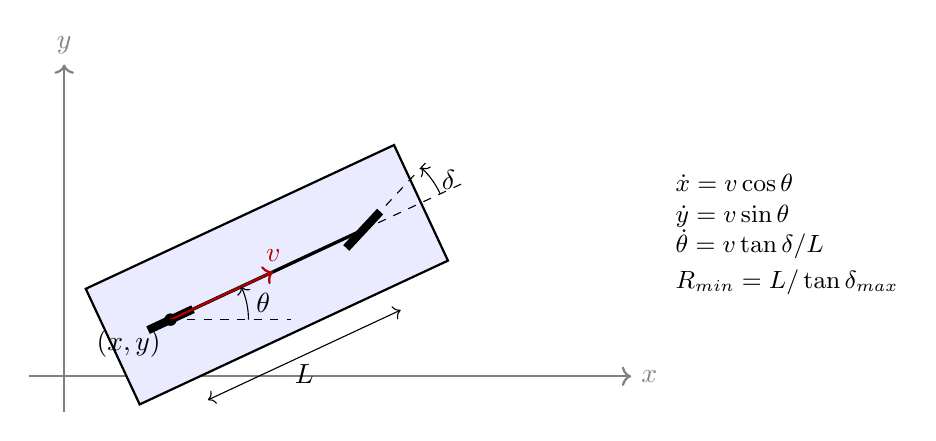
\begin{tikzpicture}[scale=0.9]
\draw[->,thick,gray] (-0.5,0) -- (8,0) node[right]{$x$};
\draw[->,thick,gray] (0,-0.5) -- (0,4.4) node[above]{$y$};
\begin{scope}[shift={(1.5,0.8)}, rotate=25]
  \draw[thick, fill=blue!8] (-0.9,-0.9) rectangle (3.9,0.9);
  \draw[very thick] (0,0) -- (3,0);
  \draw[line width=3pt] (-0.35,0) -- (0.35,0);
  \begin{scope}[shift={(3,0)}, rotate=22] \draw[line width=3pt] (-0.35,0) -- (0.35,0); \draw[dashed] (0,0) -- (1.4,0); \end{scope}
  \fill (0,0) circle (2.5pt) node[below left]{$(x,y)$};
  \draw[dashed] (3,0) -- (4.6,0);
  \draw[->] (4.2,0) arc (0:22:1.2) node[midway,right]{$\delta$};
  \draw[<->] (0,-1.25) -- (3,-1.25) node[midway,below]{$L$};
  \draw[->,thick,red!70!black] (0,0) -- (1.6,0) node[above]{$v$};
\end{scope}
\draw[dashed] (1.5,0.8) -- (3.2,0.8);
\draw[->] (2.6,0.8) arc (0:25:1.1) node[midway,right]{$\theta$};
\node[align=left, font=\small] at (10.2,2.0) {$\dot x = v\cos\theta$\\ $\dot y = v\sin\theta$\\ $\dot\theta = v\tan\delta / L$\\[2pt] $R_{min} = L/\tan\delta_{max}$};
\end{tikzpicture}
\caption{Kinematic bicycle model of the Ackermann car (reference point: rear-axle centre)}
\label{fig:bicycle}
\end{figure}

\subsection{A* and Hybrid A*}
A* expands nodes in order of $f(n) = g(n) + h(n)$, where $g$ is the cost from the start and $h$ an estimate of the remaining cost. If $h$ never overestimates (it is \emph{admissible}), the first path found to the goal is optimal [8]. Hybrid A* [4] keeps the same priority queue, but a node is a continuous pose $(x, y, \theta)$, and its children are produced by integrating Eq.~(\ref{eq:bicycle}) for a fixed arc length with a set of steering angles, forward and in reverse (motion primitives). A closed set over discretised cells ($0.5~\text{m} \times 0.5~\text{m} \times 5^\circ$) prevents re-expanding similar poses. Our step cost is
\begin{equation}
c = \ell\,(1 + 0.6\,[\text{reverse}]) + 0.4\,|\delta| + 0.8\,|\delta - \delta_{prev}| + 6\,[\text{gear change}],
\label{eq:cost}
\end{equation}
where $\ell = 1$~m is the primitive length and $[\cdot]$ is 1 when the condition holds. The heuristic is $h = \max(d_{Euclid}, d_{Dijkstra})$, where $d_{Dijkstra}$ is the obstacle-aware shortest distance on a 0.5~m grid, computed once from the goal.

\subsection{Path-tracking control}
\textbf{Pure Pursuit} [11] chooses a look-ahead point at distance $L_d$ on the path and steers along the circular arc through it. If $\alpha$ is the angle between the direction of motion and the look-ahead point,
\begin{equation}
\kappa = \frac{2\sin\alpha}{L_d}, \qquad \delta = \sigma \arctan(L\kappa), \qquad L_d = \max(1.6, 0.8|v|),
\label{eq:pp}
\end{equation}
where $\sigma = +1$ forward and $\sigma = -1$ in reverse. In reverse, the direction of motion is $\theta + \pi$ and $\dot\theta$ changes sign with $v$ in Eq.~(\ref{eq:bicycle}).

\textbf{Stanley} [12] uses the heading error $\psi_e$ and the cross-track error $e$ of the front axle:
\begin{equation}
\delta = \psi_e + \arctan\frac{k\,e}{k_s + |v|}, \qquad k = 1.2,\; k_s = 0.5.
\label{eq:stanley}
\end{equation}

\textbf{PID speed control.} The speed loop computes an acceleration command
\begin{equation}
a_{cmd}(t) = K_p e_v(t) + K_i \int_0^t e_v\,d\tau - K_d \frac{dv}{dt}, \qquad e_v = v_{ref} - v,
\label{eq:pid}
\end{equation}
with $K_p = 1.8$, $K_i = 0.6$, $K_d = 0.05$, saturation to $[-3, 1.5]$~m/s$^2$ and anti-windup. The drivetrain is modelled as a first-order lag $\tau\dot a = a_{cmd} - a$ with $\tau = 0.45$~s, so the plant from $a_{cmd}$ to $v$ is $G(s) = 1/(s(\tau s + 1))$.

\subsection{Time to collision and Kalman filter}
Time to collision is the time left before contact if nothing changes: $\text{TTC} = d / v_{close}$ [15]. Our reflex rule turns it around and limits the speed so that $\text{TTC} \ge T_{safe}$ (Eq.~(\ref{eq:ttc}) in Section~7.4). For localisation, a Kalman filter predicts the position from odometry ($x_k = x_{k-1} + v\,\Delta t\cos\theta$, variance $P \leftarrow P + Q\,\Delta t$) and corrects it with GPS ($K = P/(P+R)$, $x \leftarrow x + K(z - x)$, $P \leftarrow (1-K)P$) [17].

\section{System Design}
\subsection{Block diagram}
Figure~\ref{fig:block} shows the full system. The parking facility (infrastructure) reports the free slots and the outlines of parked cars, as in ISO 23374 [1]. The car's own sensors feed a Kalman filter and the reflex layer. The three agent layers turn this information into a steering angle and a speed command for the Webots \texttt{Driver} (vehicle library).

\begin{figure}[!htbp]
\centering
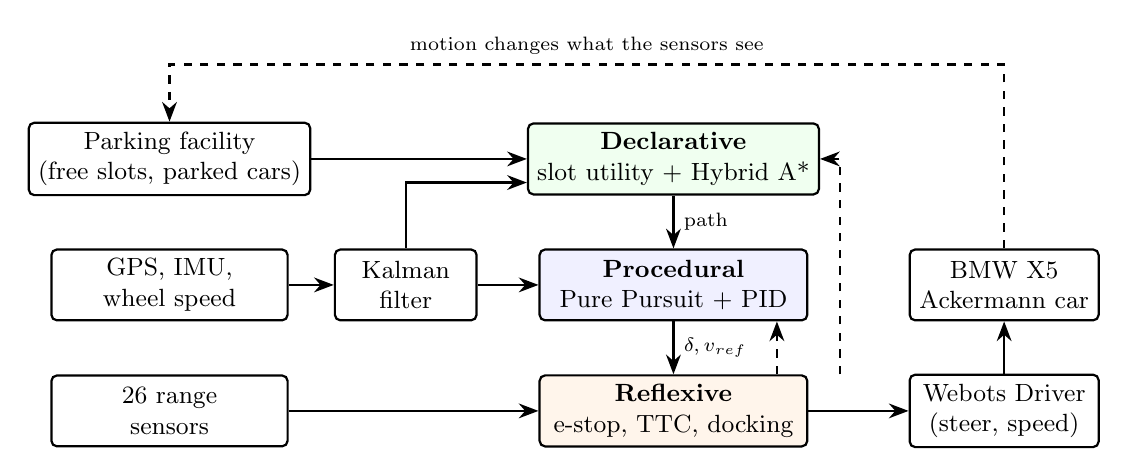
\begin{tikzpicture}
\node[box, minimum width=3.0cm] (inf) at (0,2.2) {Parking facility\\(free slots, parked cars)};
\node[box, minimum width=3.0cm] (gps) at (0,0.6) {GPS, IMU,\\wheel speed};
\node[box, minimum width=3.0cm] (rs)  at (0,-1.0) {26 range\\sensors};
\node[box, minimum width=1.8cm] (kf)  at (3.0,0.6) {Kalman\\filter};
\node[box, minimum width=3.4cm, fill=green!6]  (dec)  at (6.4,2.2) {\textbf{Declarative}\\slot utility + Hybrid A*};
\node[box, minimum width=3.4cm, fill=blue!6]   (proc) at (6.4,0.6) {\textbf{Procedural}\\Pure Pursuit + PID};
\node[box, minimum width=3.4cm, fill=orange!8] (ref)  at (6.4,-1.0) {\textbf{Reflexive}\\e-stop, TTC, docking};
\node[box, minimum width=2.4cm] (drv) at (10.6,-1.0) {Webots Driver\\(steer, speed)};
\node[box, minimum width=2.4cm] (car) at (10.6,0.6) {BMW X5\\Ackermann car};
\draw[arr] (inf) -- (dec);
\draw[arr] (gps) -- (kf);
\draw[arr] (kf) -- (proc);
\draw[arr] (kf.north) |- ([yshift=-3mm]dec.west);
\draw[arr] (dec) -- node[right,font=\scriptsize]{path} (proc);
\draw[arr] (proc) -- node[right,font=\scriptsize]{$\delta, v_{ref}$} (ref);
\draw[arr] (rs) -- (ref);
\draw[arr] (ref) -- (drv);
\draw[arr] (drv) -- (car);
\draw[arr, dashed] ([xshift=-4mm]ref.north east) -- ([xshift=-4mm]proc.south east);
\draw[arr, dashed] ([xshift=4mm]ref.north east) |- (dec.east);
\draw[arr, dashed] (car.north) |- node[above, font=\scriptsize, pos=0.75]{motion changes what the sensors see} (0,3.4) -- (inf.north);
\end{tikzpicture}
\caption[Block diagram of the valet parking system]{Block diagram of the valet parking system (dashed: reflex override and ``blocked $\rightarrow$ re-plan'' events)}
\label{fig:block}
\end{figure}

\subsection{Three-layer agent architecture}
Figure~\ref{fig:layers} shows the agent's internal structure. The layers differ in how often they run and how far ahead they look. A higher-priority (lower) layer can override the command of the layer above it, as in subsumption [5].

\begin{figure}[!htbp]
\centering
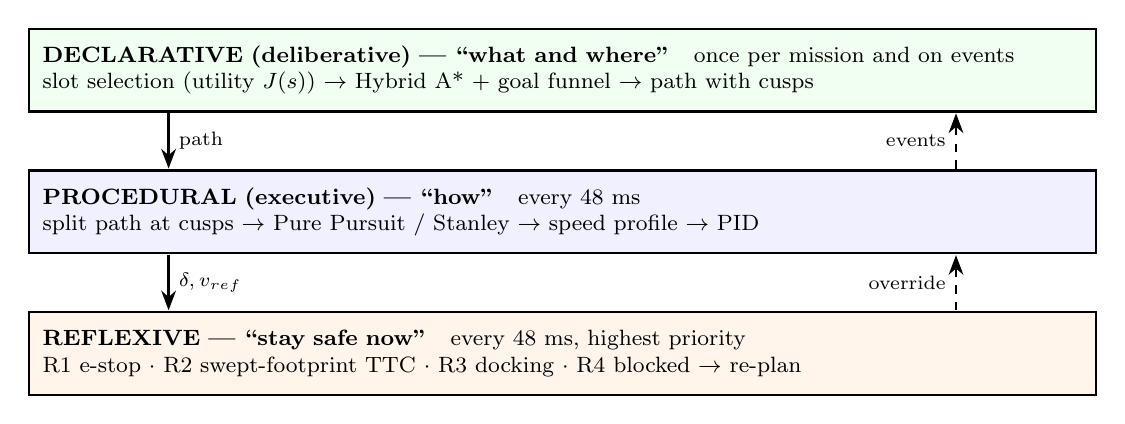
\begin{tikzpicture}[lay/.style={draw, thick, text width=13.2cm, minimum height=1.05cm, align=left, font=\footnotesize, inner sep=5pt}]
\node[lay, fill=green!6]  (d) at (0,3.6) {\textbf{DECLARATIVE (deliberative) --- ``what and where''}\quad once per mission and on events\\ slot selection (utility $J(s)$) $\rightarrow$ Hybrid A* + goal funnel $\rightarrow$ path with cusps};
\node[lay, fill=blue!6]   (p) at (0,1.8) {\textbf{PROCEDURAL (executive) --- ``how''}\quad every 48 ms\\ split path at cusps $\rightarrow$ Pure Pursuit / Stanley $\rightarrow$ speed profile $\rightarrow$ PID};
\node[lay, fill=orange!8] (r) at (0,0) {\textbf{REFLEXIVE --- ``stay safe now''}\quad every 48 ms, highest priority\\ R1 e-stop $\cdot$ R2 swept-footprint TTC $\cdot$ R3 docking $\cdot$ R4 blocked $\rightarrow$ re-plan};
\draw[arr] (-5.0,3.05) -- node[right,font=\scriptsize]{path} (-5.0,2.35);
\draw[arr] (-5.0,1.25) -- node[right,font=\scriptsize]{$\delta, v_{ref}$} (-5.0,0.55);
\draw[arr, dashed] (5.0,0.55) -- node[left,font=\scriptsize]{override} (5.0,1.25);
\draw[arr, dashed] (5.0,2.35) -- node[left,font=\scriptsize]{events} (5.0,3.05);
\end{tikzpicture}
\caption{Declarative--procedural--reflexive hierarchy of the agent (solid: commands, dashed: events)}
\label{fig:layers}
\end{figure}

\textbf{PEAS description of the agent [14].} \emph{Performance:} parked inside a free slot, accuracy, time, no contact. \emph{Environment:} parking lot, parked cars, pedestrians, other cars taking slots. \emph{Actuators:} steering angle, speed (or throttle/brake and gear). \emph{Sensors:} GPS, IMU, wheel speed, 26 range sensors, facility messages.

\subsection{Robot and environment model}
\textbf{Environment.} The lot (Fig.~\ref{fig:lot}) has four rows of 12 slots (2.8~m~$\times$~5.5~m), two 7~m aisles, a 6~m entry lane on the left, a low kerb between the back-to-back middle rows, and walls on all sides. The drop-off (start) point is at the bottom left and the pick-up zone at the top left. Parked cars are boxes of random size (4.3--4.9~m~$\times$~1.75--1.95~m), placed with random offsets of up to 0.2~m and $3^\circ$. Pedestrians walk across the aisles at 0.9--1.4~m/s.

\begin{figure}[!htbp]
\centering
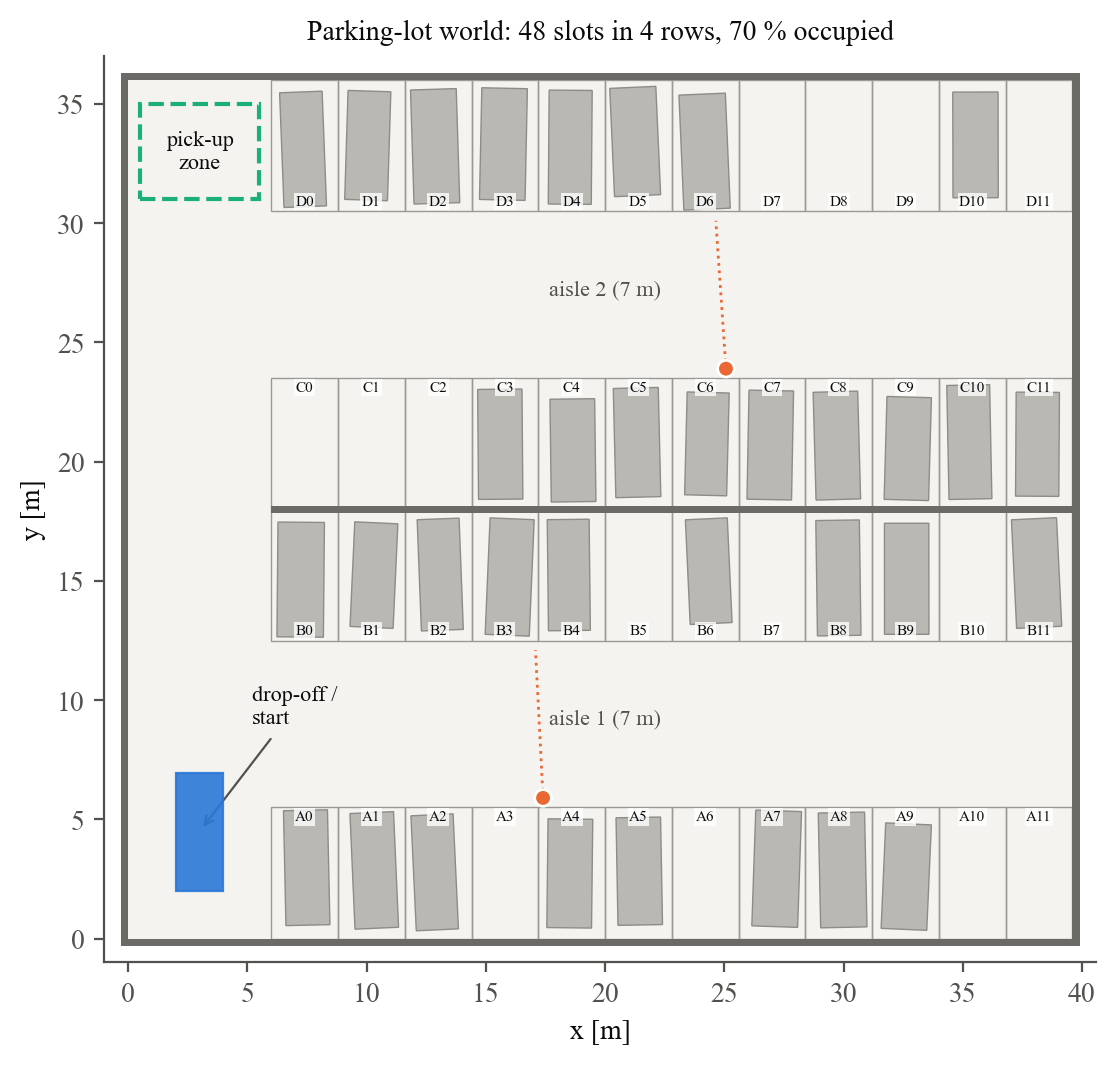
\includegraphics[width=0.62\linewidth]{fig_lot_layout.png}
\caption{Parking-lot environment (one random scenario: 70\% occupied, two pedestrian crossings)}
\label{fig:lot}
\end{figure}

\textbf{Vehicle.} Table~\ref{tab:veh} lists the vehicle parameters. They match the Webots \texttt{BmwX5} model.

\begin{table}[!htbp]
\centering
\caption{Vehicle parameters (Webots BmwX5)}
\label{tab:veh}
\renewcommand{\arraystretch}{1.2}
\begin{tabular}{|P{6cm}|C{3.2cm}|P{3.8cm}|}
\hline
\textbf{Parameter} & \textbf{Value} & \textbf{Note} \\ \hline
Wheelbase $L$ & 2.995 m & BmwX5 PROTO \\ \hline
Length $\times$ width & 4.945 m $\times$ 1.95 m & overhangs 0.95 / 1.00 m \\ \hline
Max steering $\delta_{max}$ / rate & 0.55 rad / 1.2 rad/s & planner uses 88\% \\ \hline
Min turning radius $R_{min}$ & 4.87 m & $L/\tan\delta_{max}$ \\ \hline
Speed limit forward / reverse & 2.2 / 0.9 m/s & AVP speeds $<$ 10 km/h \\ \hline
Drivetrain lag $\tau$, max accel & 0.45 s, 1.5 m/s$^2$ & first-order model \\ \hline
\end{tabular}
\end{table}

\subsection{Sensors and actuators}
\begin{figure}[!htbp]
\centering
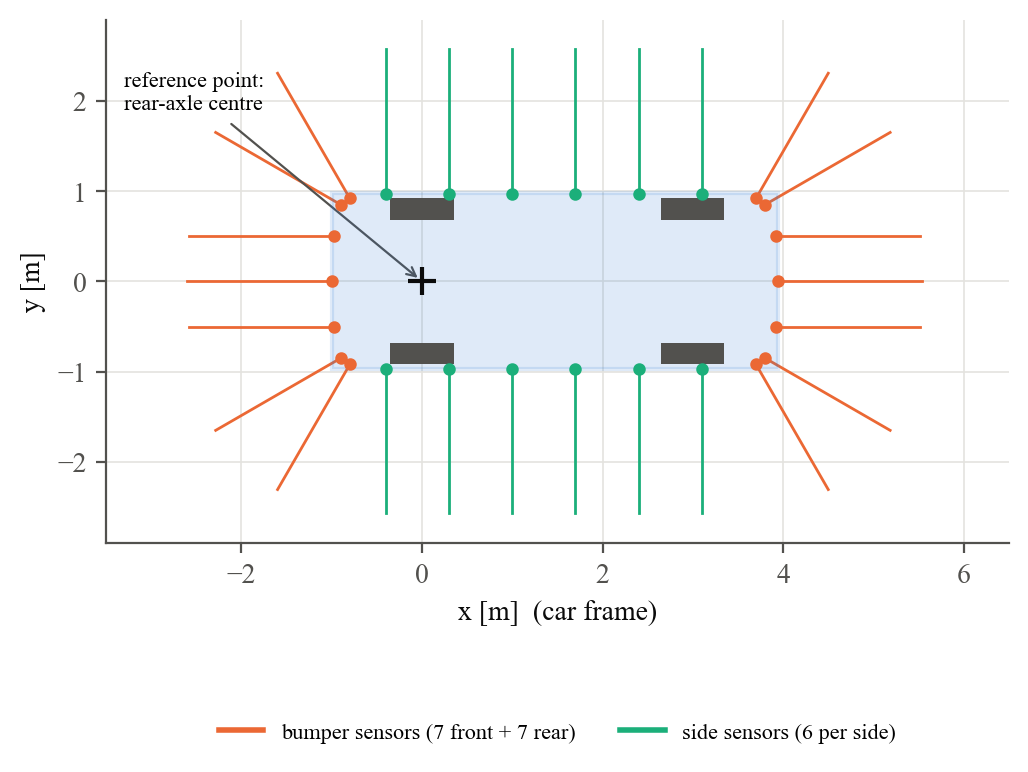
\includegraphics[width=0.66\linewidth]{fig_sensor_layout.png}
\caption{Sensor layout: 7 range sensors on each bumper and 6 on each side, mounted 0.5 m high}
\label{fig:sensors}
\end{figure}

Figure~\ref{fig:sensors} shows the 26 range sensors (Webots \texttt{DistanceSensor}, range 8~m, noise 2~cm), modelled on the 12--16 ultrasonic sensors of production park-assist systems. Each bumper has a centre sensor, two straight sensors at $\pm 0.5$~m and corner sensors at $\pm 30^\circ$ and $\pm 60^\circ$, so a 0.7~m wide pedestrian cannot hide between two rays. Six side sensors per side, spaced 0.7~m, cover the flanks of the car during a turn. A GPS (accuracy 5~cm) and an inertial unit (yaw) sit at the rear-axle centre. The actuators are the steering angle and the cruising speed of the Webots \texttt{Driver} (or throttle, brake and gear in the optional torque mode).

\subsection{Software architecture}
Figure~\ref{fig:sw} shows the code modules. The important design decision is that \texttt{valet/} is pure Python with no Webots imports. It is called by a thin Webots controller \emph{and} by the headless twin, so every algorithm is tested in both, and the Webots world is generated from the same lot model, so the two can never drift apart.

\begin{figure}[!htbp]
\centering
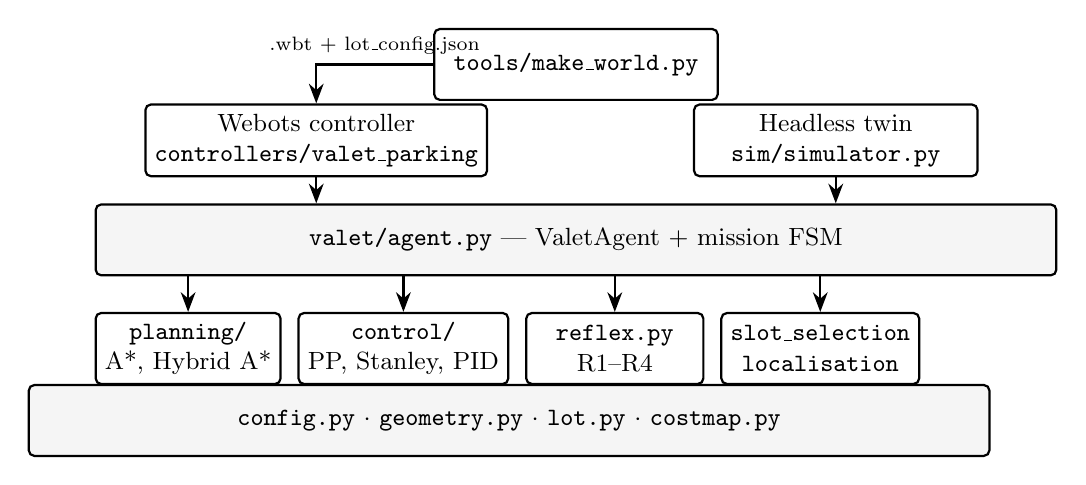
\begin{tikzpicture}[node distance=0.35cm and 0.45cm, every node/.style={font=\small}]
\node[box, minimum width=3.6cm] (wb) {Webots controller\\\texttt{controllers/valet\_parking}};
\node[box, minimum width=3.6cm, right=2.6cm of wb] (tw) {Headless twin\\\texttt{sim/simulator.py}};
\node[box, minimum width=12.2cm, below=0.8cm of $(wb)!0.5!(tw)$, fill=gray!8] (ag) {\texttt{valet/agent.py} --- ValetAgent + mission FSM};
\node[box, below=0.45cm of ag.south west, anchor=north west, minimum width=2.25cm] (pl) {\texttt{planning/}\\A*, Hybrid A*};
\node[box, right=0.2cm of pl, minimum width=2.25cm] (co) {\texttt{control/}\\PP, Stanley, PID};
\node[box, right=0.2cm of co, minimum width=2.25cm] (rf) {\texttt{reflex.py}\\R1--R4};
\node[box, right=0.2cm of rf, minimum width=2.25cm] (ss) {\texttt{slot\_selection}\\\texttt{localisation}};
\node[box, below=0.45cm of $(co)!0.5!(rf)$, minimum width=12.2cm, fill=gray!8] (base) {\texttt{config.py} $\cdot$ \texttt{geometry.py} $\cdot$ \texttt{lot.py} $\cdot$ \texttt{costmap.py}};
\node[box, above=0.5cm of $(wb)!0.5!(tw)$, minimum width=3.6cm] (mw) {\texttt{tools/make\_world.py}};
\draw[arr] (wb) -- (wb |- ag.north);
\draw[arr] (tw) -- (tw |- ag.north);
\draw[arr] (mw) -| node[above, pos=0.25, font=\scriptsize]{.wbt + lot\_config.json} (wb);
\foreach \n in {pl,co,rf,ss} \draw[arr] (\n |- ag.south) -- (\n);
\end{tikzpicture}
\caption{Software architecture: one agent package shared by Webots and the headless twin}
\label{fig:sw}
\end{figure}

\section{Methodology and Algorithms}
\subsection{Mission state machine and control cycle}
The agent is driven by the finite-state machine of Fig.~\ref{fig:fsm}. At every control step ($\Delta t = 48$~ms in Webots, 50~ms in the twin) it: (1) reads GPS, IMU, wheel speed and the 26 ranges; (2) updates the Kalman filter; (3) runs the declarative layer if the state is SELECT or PLAN; (4) runs the procedural layer to get $(\delta, v_{ref})$; (5) lets the reflex layer modify $(\delta, v_{ref})$; (6) closes the speed loop with the PID and sends the commands; and (7) logs the data.

\begin{figure}[!htbp]
\centering
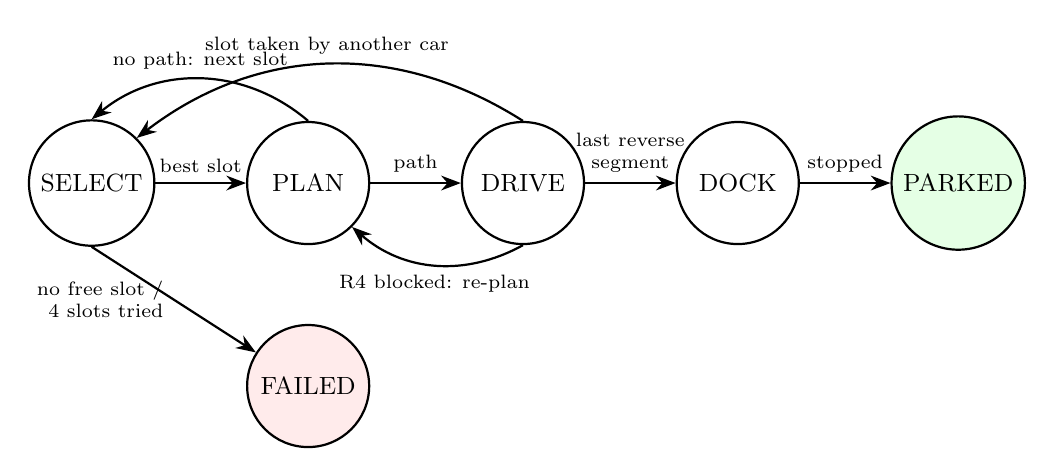
\begin{tikzpicture}[node distance=0.6cm and 1.15cm, >={Stealth[length=2.5mm]}]
\node[st] (sel) {SELECT};
\node[st, right=of sel] (pl) {PLAN};
\node[st, right=of pl] (dr) {DRIVE};
\node[st, right=of dr] (dk) {DOCK};
\node[st, right=of dk, fill=green!10] (pk) {PARKED};
\node[st, below=1.0cm of pl, fill=red!8] (fl) {FAILED};
\draw[arr] (sel) -- node[above,font=\scriptsize]{best slot} (pl);
\draw[arr] (pl) -- node[above,font=\scriptsize]{path} (dr);
\draw[arr] (dr) -- node[above,font=\scriptsize,align=center]{last reverse\\segment} (dk);
\draw[arr] (dk) -- node[above,font=\scriptsize]{stopped} (pk);
\draw[arr] (pl.north) to[bend right=40] node[above,font=\scriptsize]{no path: next slot} (sel.north);
\draw[arr] (dr.north) to[bend right=35] node[above,font=\scriptsize]{slot taken by another car} (sel.north east);
\draw[arr] (dr.south) to[bend left=35] node[below,font=\scriptsize]{R4 blocked: re-plan} (pl.south east);
\draw[arr] (sel.south) -- node[left,font=\scriptsize,align=right]{no free slot /\\4 slots tried} (fl);
\end{tikzpicture}
\caption{Mission finite-state machine of the valet agent}
\label{fig:fsm}
\end{figure}

\subsection{Declarative layer: slot selection}
The agent evaluates every free slot $s$ with the cost (negative utility)
\begin{equation}
J(s) = D_{in}(s) + w_{out}\,D_{out}(s) + w_{m}\,M(s), \qquad w_{out} = 1,\; w_m = 4~\text{m},
\label{eq:utility}
\end{equation}
where $D_{in}$ is the driving distance from the car to the slot, $D_{out}$ the driving distance from the slot to the pick-up zone, and $M(s)$ the manoeuvre difficulty: the number of occupied neighbours (0--2), plus 1 if the slot across the aisle is occupied (less room to swing the front), plus 1 for a slot at the end wall. $D_{in}$ and $D_{out}$ for \emph{all} slots come from two Dijkstra runs on the inflated grid, so ranking all 48 slots takes only a fraction of a second. The baseline policy takes the slot nearest to the car.

\subsection{Declarative layer: Hybrid A* with goal funnel}
Algorithm~\ref{alg:hybrid} gives our Hybrid A*. A pose is collision-free if every point of the car outline (sampled every 0.2~m) is more than the safety margin (0.2~m) from the nearest obstacle. The distance comes from a Euclidean distance transform of a 0.1~m occupancy grid, so each check is a few array look-ups. Primitives use 88\% of the steering limit, which leaves a reserve for the feedback controller (Section~9.6 explains why this matters). The goal is the reverse-in pose: rear bumper 0.4~m from the slot's back line, nose facing the aisle.

\begin{algorithm}[H]
\caption{Hybrid A* with slot goal funnel}
\label{alg:hybrid}
\begin{algorithmic}[1]
\Require start pose $q_s$, parking pose $q_g$, costmap $\mathcal{C}$
\Ensure drivable path with direction labels (forward / reverse)
\State $h_{map} \gets$ Dijkstra from $q_g$ on the inflated grid \Comment{obstacle-aware heuristic}
\State OPEN $\gets \{q_s\}$ with $f = h(q_s)$; CLOSED $\gets \emptyset$
\While{OPEN not empty and expansions $< N_{max}$}
  \State $n \gets$ pop node with lowest $f$; skip it if cell$(n) \in$ CLOSED; add cell$(n)$ to CLOSED
  \If{\Call{Funnel}{$n$, $q_g$}} \Comment{novelty 1}
     \State \Return path$(n)$ + straight reverse from $n$ to $q_g$
  \EndIf
  \For{each direction $d \in \{+1,-1\}$, steering $\delta \in \{-0.88\delta_{max}, \dots, +0.88\delta_{max}\}$}
     \State $q' \gets$ integrate Eq.~(\ref{eq:bicycle}) for 1 m in 0.25 m steps
     \If{all intermediate poses are free in $\mathcal{C}$}
        \State $g' \gets g(n) +$ step cost Eq.~(\ref{eq:cost}); push $q'$ with $f = g' + \max(h_{map}, d_{Euclid})$ if $g'$ improves its cell
     \EndIf
  \EndFor
\EndWhile
\State \Return failure \Comment{agent tries the next slot}
\Statex
\Function{Funnel}{$n$, $q_g$}
  \State express $n$ in the slot frame: distance along the axis $a$, lateral offset $e$, heading error $\Delta\theta$
  \State \Return $2.5 \le a \le 7$ m \textbf{and} $|e| < 0.2$ m \textbf{and} $|\Delta\theta| < 6^\circ$ \textbf{and} straight segment to $q_g$ is free
\EndFunction
\end{algorithmic}
\end{algorithm}

The baseline \textbf{grid A*} runs 8-connected A* (octile heuristic, no corner cutting) on a 0.25~m grid whose obstacles are inflated by half the car width plus the margin. It then shortens the path by line-of-sight smoothing. It drives into the slot nose-first, because it has no notion of heading or reversing.

\subsection{Procedural layer: path execution}
\begin{enumerate}[itemsep=1pt,topsep=2pt]
\item \textbf{Segmenting.} The path is split at every cusp (change of gear) into constant-direction segments.
\item \textbf{Steering.} For the active segment, the nearest waypoint is found in a moving window, and the steering angle comes from Pure Pursuit (Eq.~\ref{eq:pp}) or Stanley (Eq.~\ref{eq:stanley}). For Stanley in reverse we use the rear axle as reference and add a curvature feed-forward $\delta_{ff} = -\arctan(L\kappa)$. Without it, Stanley needs a large steady error to hold an arc.
\item \textbf{Speed profile.} $v_{ref} = \min\!\big(v_{max},\ \sqrt{1/\kappa_{ahead}},\ \sqrt{2 a_{b} (d_{end} - 0.5|v|)} + 0.1\big)$, with the cruise speed 2.2~m/s forward and 0.9~m/s in reverse, lateral acceleration below 1~m/s$^2$, and braking $a_b = 0.6$~m/s$^2$. The term $0.5|v|$ subtracts the distance covered during the drivetrain lag. Without it the car overshot every stop by about 0.35~m.
\item \textbf{Cusp handling.} At the end of a segment the car stops ($|v| < 0.08$~m/s), steers at standstill towards the next segment, and changes gear.
\item \textbf{Speed loop.} The PID of Eq.~(\ref{eq:pid}) turns $v_{ref}$ (after the reflex layer) into an acceleration command. In Webots it is sent as a cruising speed, or as throttle/brake with gear selection in torque mode.
\end{enumerate}

\textbf{Controller design and tuning.} Pure Pursuit gains: the look-ahead was swept from 1.0 to 3.0~m on test missions. Below 1.4~m the steering oscillated at the cusps, and above 2.2~m the car cut the corners of the turn into the aisle, so we use $L_d = \max(1.6, 0.8|v|)$ (1.2~m minimum in reverse, where the car is slow). For the speed PID, $K_p$ was raised until the rise time was below 1~s. $K_i$ removes the steady error caused by the drivetrain lag, and a small $K_d$ damps the overshoot. The resulting loop has a phase margin of \PhaseMargin$^\circ$ (Section~9.3).

\subsection{Reflexive layer}
Algorithm~\ref{alg:reflex} lists the reflex rules in priority order. The key quantity is the \emph{swept contact distance} $s_c$ (novelty 2). All range readings are converted into points in the car frame. The car outline, inflated by 0.2~m, is moved along the arc of the current steering angle in 0.1~m steps, and $s_c$ is the arc length at which the first point enters it. The TTC speed limit is then
\begin{equation}
v_{allow} = \max\!\Big(0,\ \frac{s_c - d_{stop}}{T_{safe}} - v_{obs}\Big), \qquad d_{stop} = 0.45~\text{m},\; T_{safe} = 2.5~\text{s},
\label{eq:ttc}
\end{equation}
where $v_{obs}$ is the closing speed of the obstacle itself, estimated from the change of $s_c$ between steps. The speed therefore falls smoothly as the car gets closer, instead of the stop--go behaviour of a fixed-distance rule.

\begin{algorithm}[H]
\caption{Reflex layer (runs every control step, after the procedural layer)}
\label{alg:reflex}
\begin{algorithmic}[1]
\Require proposed $(\delta, v_{ref})$, ranges $r_1..r_{26}$, speed $v$, state
\If{state = DOCK} \Comment{R3: close-range reactive rules inside the slot}
   \If{$r_{rear} < 0.25$ m} \Return $(\delta, 0)$ and mark the mission complete \EndIf
   \If{both side groups see a car within 1.5 m} $\delta \gets \delta + \text{clip}(0.12\,(d_{left} - d_{right}), \pm 0.08)$ \EndIf
   \State \Return $(\delta, v_{ref})$
\EndIf
\State $s_c \gets$ swept contact distance along the arc of $\delta$ in the direction of $v_{ref}$
\If{$s_c < d_{stop}$} $v_{ref} \gets 0$ \Comment{R1 emergency stop}
\Else\ $|v_{ref}| \gets \min(|v_{ref}|, v_{allow})$ from Eq.~(\ref{eq:ttc}) \Comment{R2 TTC limit}
\EndIf
\If{held at $v \approx 0$ for more than 4 s} \Comment{R4}
   \State add a 0.9 m box at the contact point; re-plan (budget 12\,000 nodes); keep the old path if no route exists
\EndIf
\State \Return $(\delta, v_{ref})$
\end{algorithmic}
\end{algorithm}

\subsection{Localisation}
The raw GPS position is fused with dead reckoning from the wheel speed and the IMU heading by the Kalman filter of Section~5.5 ($R = 0.15^2$~m$^2$, $Q = 0.03^2$~m$^2$/s). A 5$\sigma$ innovation gate rejects outliers. The yaw comes straight from the IMU, so $x$ and $y$ decouple into two scalar filters, which are exact and cost almost nothing.

\section{Simulation Setup}
\subsection{Platforms}
\textbf{Webots R2025a} [7] with the vehicle library (\texttt{BmwX5} PROTO, Ackermann steering, \texttt{Driver} API), the \texttt{Pedestrian} PROTO and a Python 3.11 controller. NumPy and SciPy are the only libraries the agent needs. \textbf{Headless twin} (\texttt{sim/simulator.py}): the same lot, car dimensions and sensor layout, with a kinematic bicycle model plus steering-rate limit and drivetrain lag, ray-cast range sensors, GPS/IMU/odometry noise and scripted pedestrians. The twin runs a mission in 1--5~s, so we could run \NMissions{} missions for statistics, which would take days in Webots. Both run the identical \texttt{ValetAgent}.

\subsection{World and parameters}
The Webots world (Fig.~\ref{fig:webots}) is generated by \texttt{tools/make\_world.py} from the same random scenario (seed) that the twin uses: floor, slot lines, walls, kerb, parked cars (as solid boxes) and pedestrians with a back-and-forth trajectory. The script also writes \texttt{lot\_config.json}, which the controller reads as the facility message. Table~\ref{tab:simparams} lists the main parameters.

\begin{figure}[!htbp]
\centering
\IfFileExists{figures/webots_screenshot.png}{%
\includegraphics[width=0.85\linewidth]{webots_screenshot.png}}{%
\fbox{\parbox[c][4cm][c]{0.8\linewidth}{\centering\small Webots screenshot of \texttt{worlds/valet\_parking.wbt}\\(save as \texttt{report/figures/webots\_screenshot.png} and recompile)}}}
\caption{Webots world: BMW X5 valet car, parked cars and a pedestrian (seed 3, 70\% occupancy)}
\label{fig:webots}
\end{figure}

\begin{table}[!htbp]
\centering
\caption{Simulation parameters}
\label{tab:simparams}
\renewcommand{\arraystretch}{1.2}
\begin{tabular}{|P{6.2cm}|P{7.2cm}|}
\hline
\textbf{Parameter} & \textbf{Value} \\ \hline
Webots basic time step / control period & 16 ms / 48 ms (twin: 50 ms) \\ \hline
Lot size, slots, aisles & 39.6 m $\times$ 36 m, 48 slots (2.8 $\times$ 5.5 m), 7 m aisles \\ \hline
Occupancy (random per seed) & 50, 70, 85, 92\% \\ \hline
GPS / heading / range / speed noise ($\sigma$) & 0.05--0.30 m / $0.5^\circ$ / 2 cm / 0.02 m/s \\ \hline
Hybrid A* grid, primitives & 0.5 m $\times$ $5^\circ$, 5 steering $\times$ 2 directions, 1 m \\ \hline
Costmap resolution, safety margin & 0.1 m, 0.2 m \\ \hline
Pedestrians & 4, speed 0.9--1.4 m/s, random start delay 0--6 s \\ \hline
Success criterion & PARKED, no contact, inside slot, $|e_{lat}| \le 0.3$ m, $|e_\theta| \le 5^\circ$ \\ \hline
Seeds per configuration & 30 (E1--E4), 15 (E5--E7) \\ \hline
\end{tabular}
\end{table}

\subsection{How to run the code}
\begin{verbatim}
pip install -r requirements.txt
python -m unittest discover -s tests
python experiments/run_experiments.py --n 30
python experiments/make_figures.py
python tools/make_world.py --seed 3     # then open .wbt
\end{verbatim}
Options such as \texttt{--planner grid}, \texttt{--law stanley}, \texttt{--reflex fixed} and \texttt{--selector nearest} switch to the baseline methods, both in the twin and in the Webots world.

\section{Results and Analysis}
All results come from the headless twin, with 30 random lots per configuration (15 for E5--E7) and a fixed seed for every mission, so every number can be reproduced. Unless stated otherwise, the agent uses Hybrid A* with the funnel, Pure Pursuit, the TTC reflex, the utility slot choice, the Kalman filter and 0.05~m GPS noise. Values are mean $\pm$ standard deviation.

\subsection{A complete mission}
Figure~\ref{fig:mission} shows a typical mission. The car leaves the drop-off point, drives forward along aisle 1 past the chosen slot, stops, changes into reverse and backs into the slot, straightening in the funnel. Figure~\ref{fig:time} shows the speed, steering and cross-track error over time. The speed follows the profile with a small overshoot. The steering stays below the limit, with a reserve from the 88\% rule, and the cross-track error stays within about 10~cm.

\begin{figure}[!htbp]
\centering
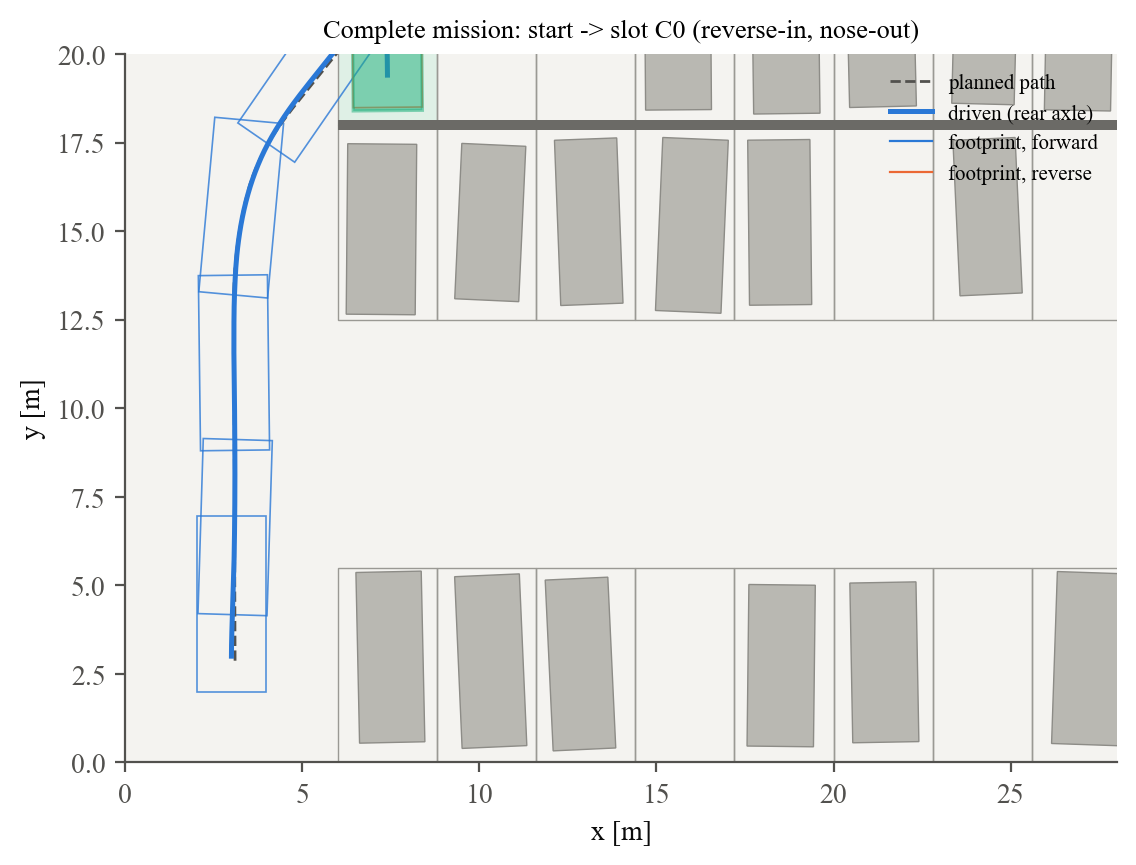
\includegraphics[width=0.62\linewidth]{fig_mission.png}
\caption{A complete mission: planned path, driven path and car footprints (blue forward, orange reverse)}
\label{fig:mission}
\end{figure}

\begin{figure}[!htbp]
\centering
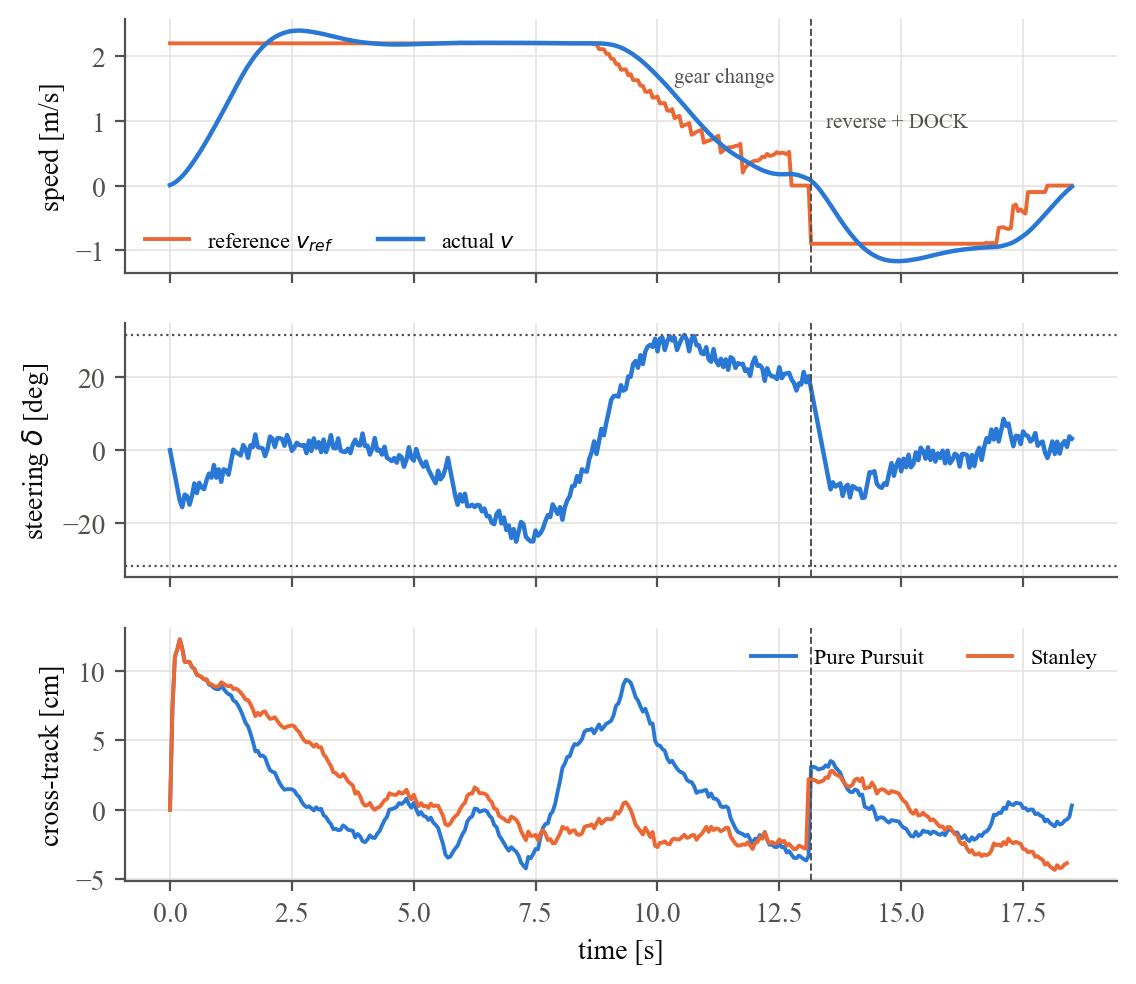
\includegraphics[width=0.64\linewidth]{fig_time_history.png}
\caption{Speed, steering angle and cross-track error during the mission of Fig.~\ref{fig:mission}}
\label{fig:time}
\end{figure}

\subsection{E1: Deliberative planners}
\begin{figure}[!htbp]
\centering
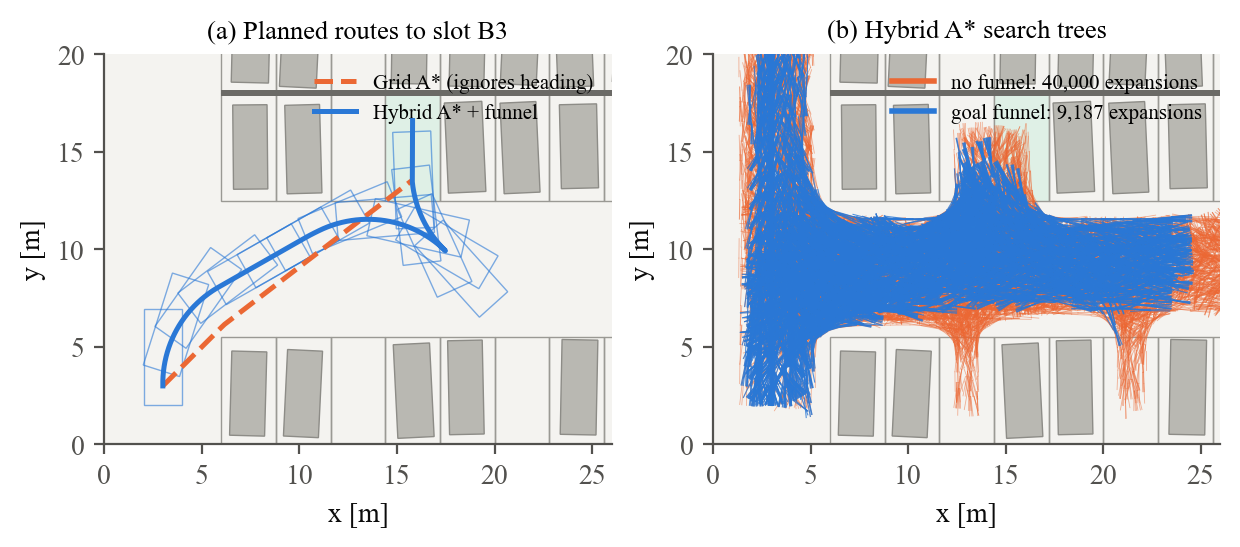
\includegraphics[width=0.88\linewidth]{fig_planner_paths.png}
\caption{(a) Grid A* and Hybrid A* routes to slot B3. (b) Search trees with and without the goal funnel}
\label{fig:paths}
\end{figure}

\begin{table}[!htbp]
\centering
\caption{E1 --- planner comparison (30 lots, 70\% occupancy)}
\label{tab:e1}
\renewcommand{\arraystretch}{1.2}
\small
\begin{tabular}{|P{3.6cm}|C{2.9cm}|C{3.1cm}|C{3.1cm}|}
\hline
\textbf{Metric} & \textbf{Grid A*} & \textbf{Hybrid A* (no funnel)} & \textbf{Hybrid A* + funnel} \\ \hline
Missions (seeds) & 30 & 30 & 30 \\ \hline
Success rate (\%) & 0.0 & 80.0 & 100.0 \\ \hline
Collisions (\%) & 0.0 & 0.0 & 0.0 \\ \hline
Planning time (s) & 0.02 $\pm$ 0.02 & 27.48 $\pm$ 24.98 & 5.08 $\pm$ 2.80 \\ \hline
Node expansions & 1075 $\pm$ 1562 & 54470 $\pm$ 49173 & 9968 $\pm$ 5291 \\ \hline
Path length (m) & 6.8 $\pm$ 7.3 & 27.5 $\pm$ 8.5 & 24.4 $\pm$ 6.6 \\ \hline
Gear changes & 0.00 $\pm$ 0.00 & 1.00 $\pm$ 0.00 & 1.17 $\pm$ 0.52 \\ \hline
Drive time, successful (s) & -- & 23.4 $\pm$ 5.3 & 24.1 $\pm$ 6.0 \\ \hline

\end{tabular}
\end{table}

Table~\ref{tab:e1} and Fig.~\ref{fig:e1} compare the planners. Grid A* plans in milliseconds, but its path has a $90^\circ$ corner into the slot that a car with $R_{min} = 4.87$~m cannot follow. When the car tried to follow it, the reflex layer prevented every contact (\EOneCollGrid\% collisions), but the car always ended up wedged against a neighbouring car, so its success rate is \EOneSuccGrid\%. This confirms that a planner must respect the vehicle's kinematics. Plain Hybrid A* needs \EOneExpNoFunnel{} expansions on average and often runs out of its 40\,000-node budget, because it must hit a small $(x, y, \theta)$ goal (Fig.~\ref{fig:paths}b). With the goal funnel, the search needs \EOneExpRatio$\times$ fewer expansions and parks successfully in \EOneSuccFunnel\% of the lots. The planning times in Table~\ref{tab:e1} were measured while seven missions ran in parallel on an 8-core laptop. Run alone, the funnel planner needs 1.65~s on average (median 1.18~s, maximum 3.4~s, 15 lots), so objective O3 is met. Paths are \EOneLenFunnel{}~m long on average with \EOneGearsFunnel{} gear changes, which is a single ``drive past and reverse in'' manoeuvre.

\begin{figure}[!htbp]
\centering
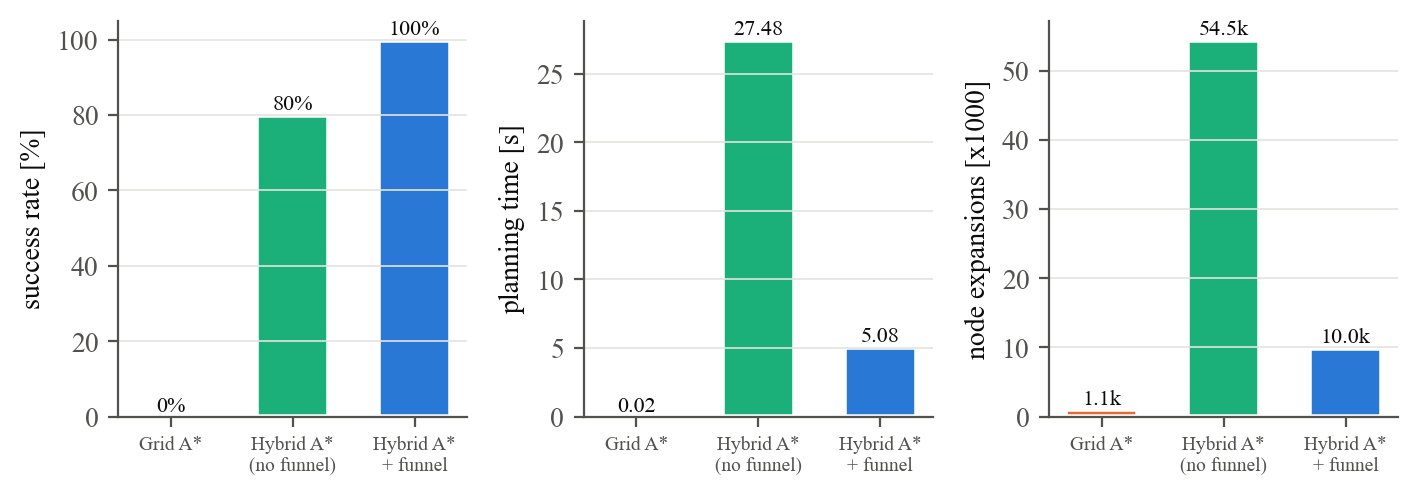
\includegraphics[width=0.8\linewidth]{fig_e1_planners.png}
\caption{E1 --- success rate, planning time and node expansions of the three planners}
\label{fig:e1}
\end{figure}

\subsection{E2: Steering laws and speed loop}
\begin{table}[!htbp]
\centering
\caption{E2 --- path-tracking laws (30 lots, Hybrid A* paths)}
\label{tab:e2}
\renewcommand{\arraystretch}{1.2}
\small
\begin{tabular}{|P{5.2cm}|C{3.6cm}|C{3.6cm}|}
\hline
\textbf{Metric} & \textbf{Pure Pursuit} & \textbf{Stanley} \\ \hline
Success rate (\%) & 100.0 & 56.7 \\ \hline
Mean $|e_{ct}|$ (cm) & 3.3 $\pm$ 1.8 & 4.3 $\pm$ 1.8 \\ \hline
Max $|e_{ct}|$ (cm) & 11.0 $\pm$ 5.5 & 13.7 $\pm$ 4.2 \\ \hline
Final $|$lateral$|$ (cm) & 4.2 $\pm$ 3.0 & 15.2 $\pm$ 7.4 \\ \hline
Final heading error (deg) & 1.18 $\pm$ 0.86 & 2.66 $\pm$ 1.27 \\ \hline
Drive time (s) & 24.1 $\pm$ 6.0 & 27.7 $\pm$ 9.1 \\ \hline

\end{tabular}
\end{table}

Both laws track well (Table~\ref{tab:e2}, Fig.~\ref{fig:time}). Pure Pursuit has a mean cross-track error of \ETwoCtePP~cm and parks with \ETwoLatPP~cm lateral and \ETwoYawPP$^\circ$ heading error, so objective O2 is met. Stanley tracks the forward part almost as well (\ETwoCteST~cm), but in reverse its rear-axle reference makes it react later. Its final errors are larger (\ETwoLatST~cm, \ETwoYawST$^\circ$), so only \ETwoSuccST\% of its missions end within the tolerance, against \ETwoSuccPP\% for Pure Pursuit. We therefore use Pure Pursuit by default. A first version of Stanley, which tracked the rear-axle path with the front axle, cut every corner by about 0.8~m. Projecting the path to the front axle fixed this (Section~7.4).

\begin{figure}[!htbp]
\centering
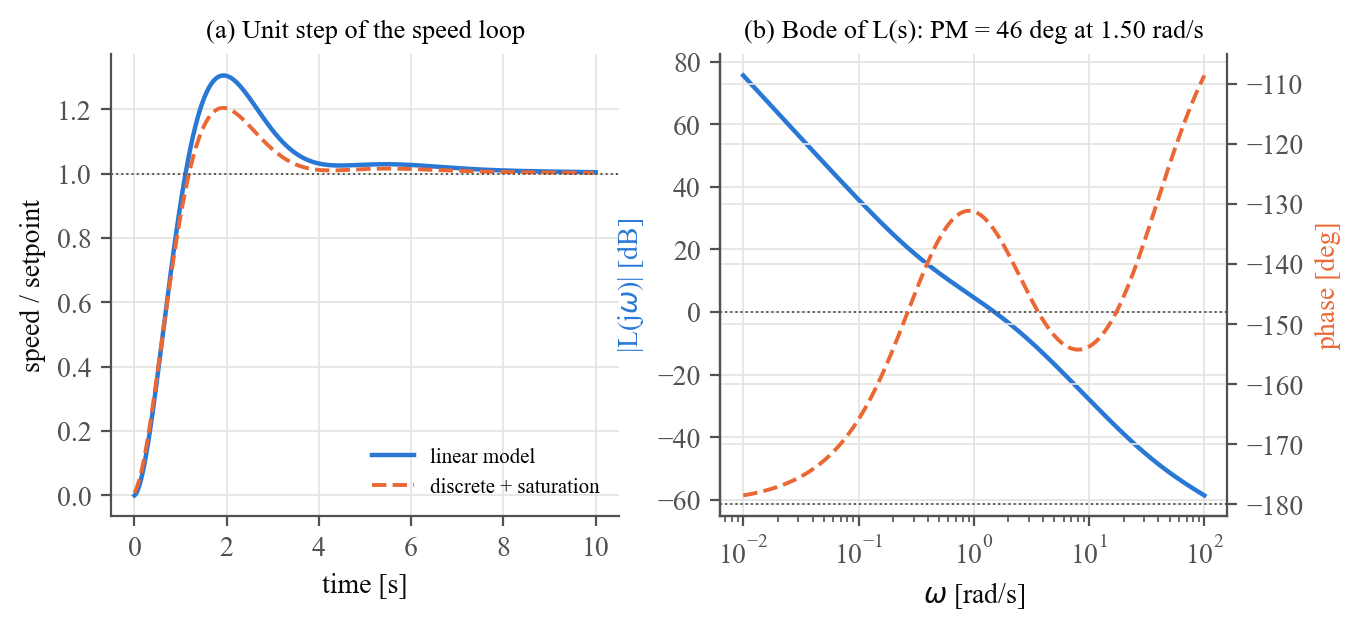
\includegraphics[width=0.8\linewidth]{fig_speed_loop.png}
\caption{Speed loop: (a) unit-step response, (b) Bode plot of the open loop $L(s) = C(s)G(s)$}
\label{fig:speed}
\end{figure}

Figure~\ref{fig:speed} analyses the speed loop in the time and frequency domain. The linear model gives a rise time of \RiseLin~s, \OvershootLin\% overshoot and a 2\% settling time of \SettleLin~s. The discrete loop with actuator saturation gives \RiseDis~s, \OvershootDis\% and \SettleDis~s. Saturation limits the acceleration, which in turn limits the integral build-up. The open loop crosses 0~dB at \CrossFreq~rad/s with a phase margin of \PhaseMargin$^\circ$, so the loop is stable with a reasonable margin. The overshoot is acceptable here because the speed profile ramps $v_{ref}$ rather than stepping it, and the overshoot appears only in the cruise phase, not at the stop.

\subsection{E3: Reflexive layer and pedestrian safety}
\begin{table}[!htbp]
\centering
\caption{E3 --- reflex designs with four crossing pedestrians (30 lots)}
\label{tab:e3}
\renewcommand{\arraystretch}{1.2}
\small
\begin{tabular}{|P{4.6cm}|C{2.7cm}|C{2.9cm}|C{2.7cm}|}
\hline
\textbf{Metric} & \textbf{No reflex} & \textbf{Fixed-distance} & \textbf{Swept TTC} \\ \hline
Success rate (\%) & 80.0 & 76.7 & 100.0 \\ \hline
Missions with contact (\%) & 20.0 & 16.7 & 0.0 \\ \hline
Min. pedestrian gap (m) & 6.31 $\pm$ 6.00 & 6.71 $\pm$ 6.13 & 6.40 $\pm$ 5.96 \\ \hline
Re-plans per mission & 0.00 $\pm$ 0.00 & 5.47 $\pm$ 15.81 & 0.03 $\pm$ 0.18 \\ \hline
Drive time, successful (s) & 21.0 $\pm$ 2.6 & 31.6 $\pm$ 40.8 & 25.8 $\pm$ 7.9 \\ \hline

\end{tabular}
\end{table}


Without a reflex layer, the car hit a pedestrian in \EThreeCollNone\% of the missions (Table~\ref{tab:e3}). The classic fixed-distance rule (stop if the straight corridor ahead is blocked within 2.5~m) reduced this to \EThreeCollFixed\%. Its remaining contacts were side-swipes during turns, where a person beside the front wing is outside the straight corridor. It also stops for parked cars that are near but not in the way, and it caused stop--go driving and long waits. The swept-footprint TTC rule reached \EThreeCollTTC\% contacts and \EThreeSuccTTC\% success (objective O4). It also drove more smoothly, because the speed falls gradually (Fig.~\ref{fig:reflex}). Developing this rule was iterative. The first version used only the bumper sensors and still had side contacts, so we added six side sensors per side. The second version could deadlock with a waiting pedestrian, so we added rule R4, which re-plans around the obstacle at the sensed contact point.

\begin{figure}[!htbp]
\centering
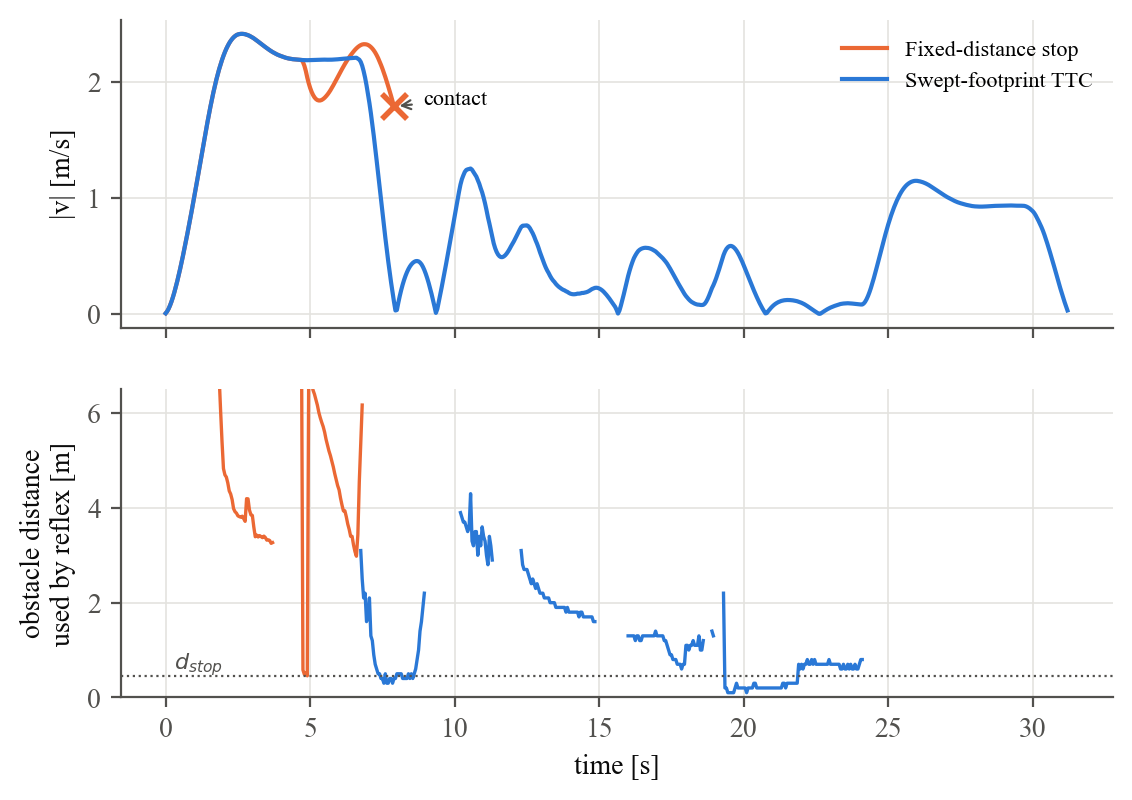
\includegraphics[width=0.64\linewidth]{fig_reflex_timeline.png}
\caption{Same lot and pedestrians: speed and obstacle distance seen by the fixed-distance and TTC reflexes}
\label{fig:reflex}
\end{figure}

\subsection{E4--E7: Agent decisions, noise and robustness}
\begin{table}[!htbp]
\centering
\caption{E4 --- slot-selection policy (30 lots, 85\% occupancy)}
\label{tab:e4}
\renewcommand{\arraystretch}{1.2}
\small
\begin{tabular}{|P{5.2cm}|C{3.6cm}|C{3.6cm}|}
\hline
\textbf{Metric} & \textbf{Nearest slot} & \textbf{Utility agent} \\ \hline
Success rate (\%) & 96.7 & 100.0 \\ \hline
Valet cycle length (m) & 54.9 $\pm$ 9.1 & 50.7 $\pm$ 7.5 \\ \hline
Parking path length (m) & 24.6 $\pm$ 5.4 & 28.6 $\pm$ 8.8 \\ \hline
Planning time (s) & 4.57 $\pm$ 1.34 & 5.55 $\pm$ 2.92 \\ \hline
Drive time (s) & 24.6 $\pm$ 5.8 & 25.6 $\pm$ 6.6 \\ \hline

\end{tabular}
\end{table}

\textbf{E4 slot selection.} The utility agent picks a different slot from the nearest-slot rule in 14 of the 30 lots, typically one in the middle rows that is a little further from the drop-off but much closer to the pick-up zone, or one with free neighbours. Over the whole valet cycle (drive in + drive out), it saves \EFourCycleGain\% of the distance (Table~\ref{tab:e4}, Fig.~\ref{fig:e4e6}b) without lowering the success rate.

\begin{table}[!htbp]
\centering
\caption{E5 --- GPS noise: raw GPS vs Kalman-filtered pose (15 lots per level)}
\label{tab:e5}
\renewcommand{\arraystretch}{1.2}
\small
\begin{tabular}{|C{2.2cm}|C{2.6cm}|C{2.6cm}|C{2.6cm}|C{2.6cm}|}
\hline
\textbf{GPS $\sigma$ (m)} & \textbf{Success raw (\%)} & \textbf{Success KF (\%)} & \textbf{$|$lat$|$ raw (cm)} & \textbf{$|$lat$|$ KF (cm)} \\ \hline
0.00 & 100 & 100 & 3.5 & 3.7 \\ \hline
0.05 & 100 & 100 & 4.3 & 4.2 \\ \hline
0.10 & 87 & 93 & 5.8 & 5.1 \\ \hline
0.20 & 60 & 100 & 7.8 & 4.2 \\ \hline
0.30 & 20 & 100 & 14.7 & 4.4 \\ \hline

\end{tabular}
\end{table}

\textbf{E5 sensor noise.} With raw GPS the controller steers on noise. At $\sigma = 0.2$~m success falls to \EFiveRawTwo\%, and at 0.3~m to \EFiveRawThree\%, mostly because the final lateral error exceeds the tolerance. With the Kalman filter, success stays at \EFiveKFTwo\% and \EFiveKFThree\% (Table~\ref{tab:e5}, Fig.~\ref{fig:noise}). This matters for real cars, where GPS in a car park is poor.

\begin{figure}[!htbp]
\centering
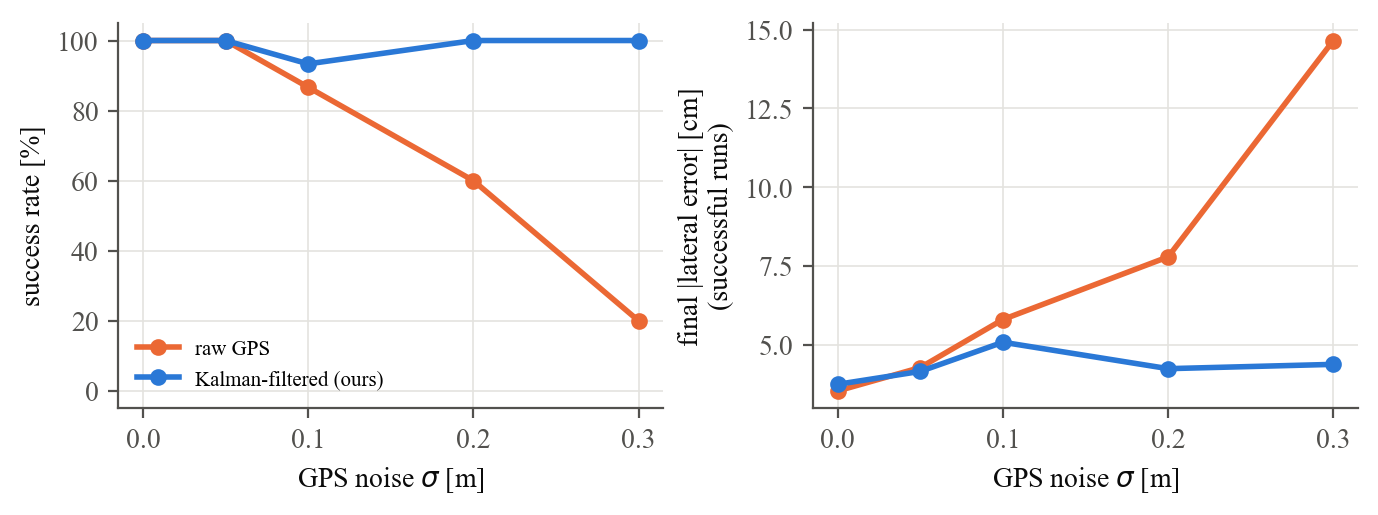
\includegraphics[width=0.75\linewidth]{fig_e5_noise.png}
\caption{E5 --- success rate and final lateral error against GPS noise}
\label{fig:noise}
\end{figure}

\begin{table}[!htbp]
\centering
\caption{E6 / E7 --- lot occupancy and the ``slot taken'' event (15 lots each)}
\label{tab:e6}
\renewcommand{\arraystretch}{1.2}
\small
\begin{tabular}{|P{3.4cm}|C{1.3cm}|C{2.3cm}|C{3.0cm}|C{2.8cm}|}
\hline
\textbf{Scenario} & \textbf{Runs} & \textbf{Success (\%)} & \textbf{Planning time (s)} & \textbf{Drive time (s)} \\ \hline
50\% & 15 & 100 & 5.79 $\pm$ 5.11 & 22.4 $\pm$ 3.6 \\ \hline
70\% & 15 & 100 & 5.27 $\pm$ 2.62 & 23.1 $\pm$ 3.7 \\ \hline
85\% & 15 & 100 & 5.15 $\pm$ 2.34 & 23.4 $\pm$ 4.4 \\ \hline
92\% & 15 & 93 & 5.85 $\pm$ 2.77 & 28.7 $\pm$ 8.5 \\ \hline
70\% + slot taken & 15 & 100 & 9.55 $\pm$ 3.20 & 29.2 $\pm$ 7.5 \\ \hline

\end{tabular}
\end{table}

\textbf{E6 occupancy and E7 dynamic events.} Success stays high from 50\% to 92\% occupancy (Table~\ref{tab:e6}, Fig.~\ref{fig:e4e6}a). Fuller lots give fewer free slots, and often only harder ones, so planning takes longer. In E7, another car takes the agent's chosen slot 4--8~s into the mission. The facility message moves the state machine back to SELECT, the agent chooses the next-best slot and re-plans from its current pose, with \ESevenSucc\% success.

\begin{figure}[!htbp]
\centering
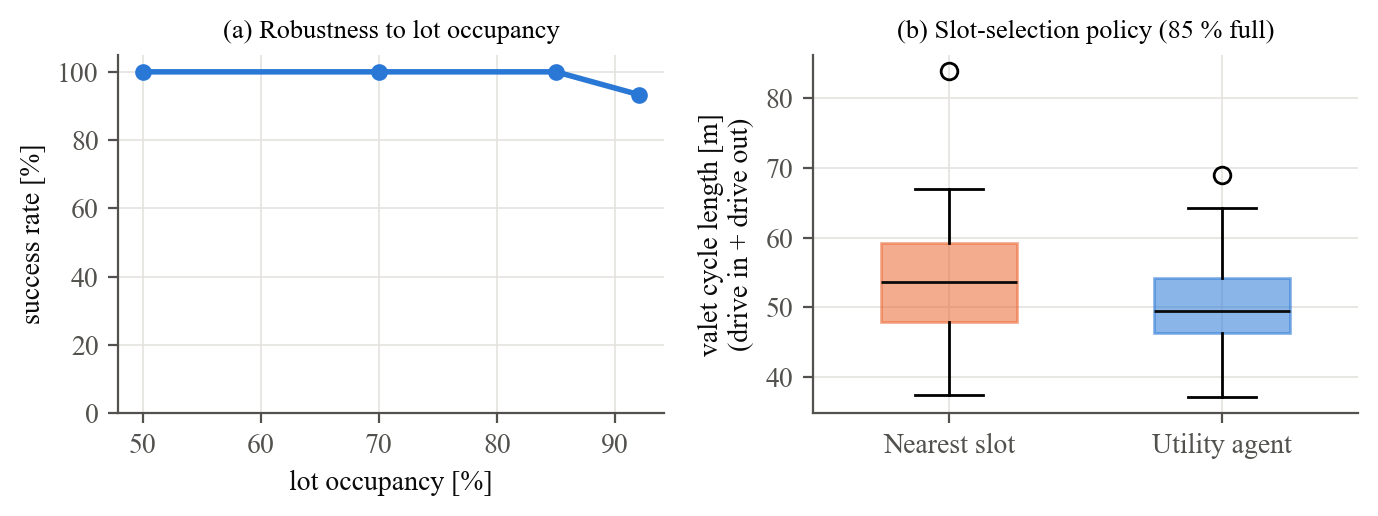
\includegraphics[width=0.75\linewidth]{fig_e4_e6.png}
\caption{(a) Success rate against lot occupancy (E6). (b) Valet cycle length for the two slot policies (E4)}
\label{fig:e4e6}
\end{figure}

\subsection{Parking accuracy, and what did not work}
Over all successful default missions the final lateral error is about 4~cm and the heading error about $1.2^\circ$ (Tables~\ref{tab:e1} and~\ref{tab:e2}), well inside the slot, which leaves 0.42~m clearance on each side.

\textbf{Honest discussion of limits.}
\begin{itemize}[itemsep=1pt,topsep=2pt]
\item \textbf{Things that failed first and how we fixed them.} (i) Planning with the full steering lock left no reserve for feedback, and the car ended up to $10^\circ$ crooked. Using 88\% of the limit fixed it. (ii) The car overshot every stop by 0.35~m until the speed profile accounted for the drivetrain lag. (iii) A funnel that accepted poses deep inside the slot gave too short a straight segment for the heading to settle, so we set a minimum length of 2.5~m.
\item \textbf{Remaining failures.} The default agent did not fail in E1--E4. The few failures in E5 and E6 (one lot each, at 0.10~m noise and at 92\% occupancy) are missions where the final heading error just exceeded $5^\circ$ or where the only remaining slot needed a long multi-shunt manoeuvre.
\item \textbf{Twin vs Webots.} The batch statistics come from the kinematic twin. Webots adds tyre slip and suspension, which can make the reverse slightly less accurate. The live Webots demonstration uses the same controller, but its run-to-run statistics would need many more runs than we could do in the project time.
\item \textbf{Python speed.} Planning takes 1--3.5~s in Python. A C++ implementation, as in industry stacks, would be about 50 times faster.
\item \textbf{Pedestrian model.} Our pedestrians are scripted and courteous. Real people can be faster or behave unpredictably, which needs a prediction model.
\end{itemize}

\Needspace{10\baselineskip}
\section{Contribution}
\renewcommand{\arraystretch}{1.25}
{\small\begin{longtable}{|c|P{2.9cm}|P{8.0cm}|P{1.7cm}|}
\caption{Technical contribution of each member}\label{tab:contrib}\\
\hline
\textbf{S. No.} & \textbf{Name and SAP ID} & \textbf{Technical contribution (modules / algorithms / code files / experiments)} & \textbf{Report sections + signature} \\ \hline
\endfirsthead
\hline
\textbf{S. No.} & \textbf{Name and SAP ID} & \textbf{Technical contribution} & \textbf{Sections + signature} \\ \hline
\endhead
1 & Saurabh Kumar (500124288), team lead & Parking-lot model and random scenario generator (\texttt{valet/lot.py}); occupancy grid and distance-transform collision check (\texttt{valet/costmap.py}); Webots world generator (\texttt{tools/make\_world.py}: slots, walls, parked cars, BmwX5 with 26 sensors, pedestrians); Webots controller (\texttt{controllers/valet\_parking}); live Webots demo; Fig.~\ref{fig:lot}, Fig.~\ref{fig:webots}. & Abstract, 1, 2, 13 \newline\newline \\ \hline
2 & Naman Chanana (500119485) & Grid A* baseline with octile heuristic and line-of-sight smoothing (\texttt{valet/planning/grid\_astar.py}); Hybrid A* with Ackermann motion primitives, Dijkstra heuristic and the slot goal funnel (\texttt{hybrid\_astar.py}, novelty 1); path class and cusp splitting (\texttt{path.py}); unit tests; experiment E1, Fig.~\ref{fig:paths}, Fig.~\ref{fig:e1}. & 3, 4 \newline\newline \\ \hline
3 & Anirvan Ranjan (500119330) & Three-layer agent and mission state machine with slot-taken and blocked events (\texttt{valet/agent.py}); utility-based slot selection (\texttt{slot\_selection.py}, novelty 3); GPS--odometry Kalman filter (\texttt{localisation.py}); experiments E4, E5, E7; Fig.~\ref{fig:layers}, \ref{fig:fsm}. & 5, 6 \newline\newline \\ \hline
4 & Aditya Pratap Singh Sisodia (500121985) & PID with anti-windup (\texttt{control/pid.py}); Pure Pursuit and Stanley for forward and reverse driving, incl.\ front-axle projection and curvature feed-forward (\texttt{control/steering.py}); path tracker with lag-aware speed profile and cusp handling (\texttt{control/tracker.py}); gain tuning, Bode/step analysis; experiment E2; Fig.~\ref{fig:time}, \ref{fig:speed}; Webots controller test. & 7, 8 \newline\newline \\ \hline
5 & Priyal Sharma (500122041) & Reflexive layer R1--R4 with the swept-footprint TTC rule (\texttt{valet/reflex.py}, novelty 2); headless simulator twin with bicycle model, ray-cast sensors and pedestrians (\texttt{sim/}); Monte Carlo runner and figure/table generation (\texttt{experiments/}); experiments E3, E6; Fig.~\ref{fig:reflex}--\ref{fig:e4e6}. & 9, 12, Appendix \newline\newline \\ \hline
\end{longtable}}
\renewcommand{\arraystretch}{1.2}

Every claim above can be traced to the commit history of the group repository (Appendix): each file was committed by the member listed above from his or her own account. All members took part in the integration tests, the recorded meetings and the demonstration video.

\section{Co-learning Reflection}
\member{Saurabh Kumar:} On my own I learned how Webots builds a vehicle from the \texttt{Car} PROTO and how the \texttt{Driver} API differs from ordinary motor control, for example that the steering angle is positive to the right. Generating the world from Python instead of drawing it by hand was my idea, and it saved us when the lot layout changed three times. From Naman I learned how Hybrid A* uses motion primitives, and from Priyal how a distance transform makes collision checks fast. I taught the team the Webots workflow and how to read the controller console when the car misbehaved.

\member{Naman Chanana:} I studied A*, Reeds--Shepp curves and the Hybrid A* paper on my own. The hardest part was seeing why the search was slow, and drawing the search tree (Fig.~\ref{fig:paths}b) showed that it wasted most nodes near the slot, which led to the goal-funnel idea. From Aditya I learned why the planner must leave a steering reserve for the controller, and from Anirvan how a state machine handles failures. I explained admissible heuristics and the cost function to the team before the viva practice.

\member{Anirvan Ranjan:} I learned the agent types of Russell and Norvig and the three-layer architecture by reading on my own, and then turned them into one \texttt{step()} function that every layer plugs into. Writing the utility function taught me that the ``best'' slot depends on the whole valet cycle, not only on the drive in. From Priyal I learned how to design a fair experiment with fixed seeds, and from Aditya the basics of a Kalman filter. I taught the others how the layers pass commands and events, so that each of us could debug our own module inside the full agent.

\member{Aditya Pratap Singh Sisodia:} On my own I learned Pure Pursuit and Stanley, and why reversing flips the sign of the steering. I found out the hard way that Stanley must track the front-axle path, after it cut every corner by 0.8~m. I also learned to read a Bode plot for a real loop and to explain overshoot from the drivetrain lag. From Saurabh I learned how Webots runs a controller, and from Naman how the planner's cusps define my segments. I taught the team how to tune a PID and how to read the tracking plots.

\member{Priyal Sharma:} I learned ray casting, time to collision and Monte Carlo evaluation on my own. The most useful lesson was that a good-looking demo can hide failures: the first pedestrian tests showed side-swipes that we only found by running hundreds of missions and checking every contact. From Anirvan I learned the agent's event handling, which I used for the blocked-replan rule, and from Saurabh the sensor modelling in Webots. I taught the team how to run the experiment scripts and regenerate all figures with one command.

\section{Conclusion and Future Scope}
\textbf{Main findings.} We built a complete autonomous valet parking agent, organised as a declarative--procedural--reflexive hierarchy, that runs in Webots and in a headless twin. Over \NMissions{} simulated missions:
\begin{enumerate}[itemsep=1pt,topsep=2pt]
\item Kinematic planning is essential. Grid A* succeeded in \EOneSuccGrid\% of the lots and Hybrid A* in \EOneSuccFunnel\%, and the goal funnel made Hybrid A* \EOneTimeRatio$\times$ faster.
\item Pure Pursuit with lag-aware speed control parks within a few centimetres and about $1^\circ$.
\item The swept-footprint TTC reflex reduced pedestrian contacts to \EThreeCollTTC\% (fixed-distance rule: \EThreeCollFixed\%) and still completed \EThreeSuccTTC\% of missions.
\item A utility-based agent shortens the valet cycle by \EFourCycleGain\%, and a simple Kalman filter makes the system robust to 0.3~m GPS noise.
\end{enumerate}

\textbf{Industrial use.} The architecture matches infrastructure-supported AVP as standardised in ISO 23374 [1]. The facility provides the free slots and parked-car outlines, and the vehicle plans and executes the manoeuvre with its own safety layer. The same agent can park cars in factory yards and ports, return rental cars, or move a robotaxi to a charger.

\textbf{Moving to a real robot.} (1) Replace the GPS by indoor localisation (lidar/camera map matching or facility beacons), keeping the Kalman filter interface. (2) Replace the range sensors by the car's ultrasonic sensors or a lidar, which only changes the conversion to points in \texttt{reflex.py}. (3) Port the planner to C++ for 50--100$\times$ speed. (4) Add a dynamic vehicle model and tyre slip to the controller. (5) Start on a 1:10 scale car (e.g.\ F1TENTH) before a full-size vehicle.

\textbf{Future scope.} Parallel and angled parking; analytic Reeds--Shepp expansion inside Hybrid A*; prediction of pedestrian motion; several valet cars sharing the lot with reservation of aisles; and retrieval missions from the slot to the pick-up zone.

\section*{References}
\addcontentsline{toc}{section}{References}
\begin{enumerate}[label={[\arabic*]},leftmargin=*,itemsep=2pt]
\item \textit{Intelligent Transport Systems --- Automated Valet Parking Systems (AVPS) --- Part 1: System Framework, Requirements for Automated Driving and for Communications Interface}, ISO 23374-1:2023, International Organization for Standardization, Geneva, Switzerland, 2023.
\item Robert Bosch GmbH, ``Bosch and Mercedes-Benz: driverless parking approved by authorities,'' press release, Stuttgart, Germany, 2022.
\item \textit{Taxonomy and Definitions for Terms Related to Driving Automation Systems for On-Road Motor Vehicles}, SAE Standard J3016\_202104, SAE International, 2021.
\item D. Dolgov, S. Thrun, M. Montemerlo, and J. Diebel, ``Path planning for autonomous vehicles in unknown semi-structured environments,'' \textit{International Journal of Robotics Research}, vol. 29, no. 5, pp. 485--501, 2010.
\item R. A. Brooks, ``A robust layered control system for a mobile robot,'' \textit{IEEE Journal on Robotics and Automation}, vol. 2, no. 1, pp. 14--23, 1986.
\item E. Gat, ``On three-layer architectures,'' in \textit{Artificial Intelligence and Mobile Robots}, D. Kortenkamp, R. P. Bonasso, and R. Murphy, Eds. Menlo Park, CA, USA: AAAI Press, 1998, pp. 195--210.
\item O. Michel, ``Webots: Professional mobile robot simulation,'' \textit{International Journal of Advanced Robotic Systems}, vol. 1, no. 1, pp. 39--42, 2004.
\item P. E. Hart, N. J. Nilsson, and B. Raphael, ``A formal basis for the heuristic determination of minimum cost paths,'' \textit{IEEE Transactions on Systems Science and Cybernetics}, vol. 4, no. 2, pp. 100--107, 1968.
\item J. A. Reeds and L. A. Shepp, ``Optimal paths for a car that goes both forwards and backwards,'' \textit{Pacific Journal of Mathematics}, vol. 145, no. 2, pp. 367--393, 1990.
\item B. Paden, M. \v{C}\'{a}p, S. Z. Yong, D. Yershov, and E. Frazzoli, ``A survey of motion planning and control techniques for self-driving urban vehicles,'' \textit{IEEE Transactions on Intelligent Vehicles}, vol. 1, no. 1, pp. 33--55, 2016.
\item R. C. Coulter, ``Implementation of the pure pursuit path tracking algorithm,'' Robotics Institute, Carnegie Mellon University, Pittsburgh, PA, USA, Tech. Rep. CMU-RI-TR-92-01, 1992.
\item S. Thrun \textit{et al.}, ``Stanley: The robot that won the DARPA Grand Challenge,'' \textit{Journal of Field Robotics}, vol. 23, no. 9, pp. 661--692, 2006.
\item J. M. Snider, ``Automatic steering methods for autonomous automobile path tracking,'' Robotics Institute, Carnegie Mellon University, Pittsburgh, PA, USA, Tech. Rep. CMU-RI-TR-09-08, 2009.
\item S. Russell and P. Norvig, \textit{Artificial Intelligence: A Modern Approach}, 4th ed. Hoboken, NJ, USA: Pearson, 2020.
\item J. C. Hayward, ``Near-miss determination through use of a scale of danger,'' \textit{Highway Research Record}, no. 384, 1972.
\item R. Rajamani, \textit{Vehicle Dynamics and Control}, 2nd ed. New York, NY, USA: Springer, 2012.
\item S. Thrun, W. Burgard, and D. Fox, \textit{Probabilistic Robotics}. Cambridge, MA, USA: MIT Press, 2005.
\end{enumerate}

\section*{Appendix: Links and Logs}
\addcontentsline{toc}{section}{Appendix: Links and Logs}
\textbf{GitHub repository:} \url{https://github.com/<team-lead>/g14-valet-parking} \\
\textbf{YouTube video (Unlisted):} \url{https://youtu.be/<video-id>}

\textbf{Repository contents.} \texttt{valet/} (agent: planners, controllers, reflex layer, slot selection, localisation), \texttt{sim/} (headless twin), \texttt{controllers/valet\_parking/} (Webots controller), \texttt{tools/make\_world.py} (Webots world generator), \texttt{experiments/} (E1--E7 and figures), \texttt{tests/} (16 unit and integration tests), \texttt{results/} (raw CSV of all missions, figures, tables).

\textbf{Meeting log}

\renewcommand{\arraystretch}{1.4}
\begin{tabular}{|c|P{1.9cm}|P{1.5cm}|P{1.9cm}|P{6.6cm}|}
\hline
\textbf{No.} & \textbf{Date} & \textbf{Duration} & \textbf{Attendees} & \textbf{Decisions} \\ \hline
1 & 15/10/2026 & & & Team lead chosen; work split into five modules; GitHub repository created \\ \hline
2 & 17/10/2026 & & & Hybrid A* chosen over grid A*; three-layer interfaces agreed; reverse-in parking policy \\ \hline
3 & 20/10/2026 & & & First full mission in the twin; stopping overshoot found and fixed \\ \hline
4 & 22/10/2026 & & & Side-swipe contacts found; swept-footprint TTC rule and side sensors added \\ \hline
5 & 24/10/2026 & & & Experiments E1--E7 run; report writing split (Writing Allocation) \\ \hline
6 & 26/10/2026 & & & Webots demo checked; slides reviewed; timed rehearsal \\ \hline
7 & 27/10/2026 & 20 min & All 5 & Recorded online presentation with live demo \\ \hline
\end{tabular}
\renewcommand{\arraystretch}{1.2}

\textbf{Peer-assessment sheet} (one sheet per member; each member rates every team-mate, 1--5)

\vspace{2pt}
Assessor name and SAP ID: \rule{8cm}{0.4pt}

\renewcommand{\arraystretch}{1.9}
\begin{tabular}{|c|P{4.4cm}|C{1.9cm}|C{2.2cm}|C{1.9cm}|C{1.7cm}|}
\hline
\textbf{No.} & \textbf{Team-mate name and SAP ID} & \textbf{Contribution (1-5)} & \textbf{Reliability / on time (1-5)} & \textbf{Helped others learn (1-5)} & \textbf{Quality of work (1-5)} \\ \hline
1 & & & & & \\ \hline
2 & & & & & \\ \hline
3 & & & & & \\ \hline
4 & & & & & \\ \hline
\end{tabular}
\renewcommand{\arraystretch}{1.2}

\vspace{0.3cm}
Signature: \rule{5cm}{0.4pt} \hfill Date: \rule{4cm}{0.4pt} \hfill \textit{(one sheet per member)}
\end{document}
